\section{Критерии качества кластеризации}

Давайте детально разберем основные метрики, используемые для оценки качества кластеризации данных.  

Выбор подходящей метрики напрямую зависит от наличия или отсутствия предварительной разметки данных и от того, задано ли количество кластеров априори или оно подбирается в процессе кластеризации.

\subsection{Критерии, не требующие разметки выборки}

\subsubsection{Среднее внутрикластерное расстояние} \hfill\\

Название этой метрики говорит само за себя: она отражает среднее расстояние между всеми парами точек внутри одного кластера.  Иными словами, мы подсчитываем сумму расстояний между всеми парами точек в каждом кластере и делим на общее количество таких пар.  

Формула метрики выглядит так:
\begin{equation*}
     F_0 = \cfrac{\displaystyle\sum_{i=1}^n \sum_{j=i}^n \rho(x_i,  x_j) I[a(  x_i)=a(x_j)]}{\displaystyle\sum_{i=1}^n \sum _ {j=i}^n I[ a(x_i)=a(x_j)]}.
\end{equation*}

В формуле учитываются и пары вида $(x_i, x_i)$, что позволяет избежать неопределенности $\frac{0}{0}$ в случае, если кластер состоит всего из одной точки.  Однако, иногда для упрощения вычислений суммирование ведется только по парам $(x_i, x_j)$, где $i < j$, при этом для случая одноточечных кластеров значение метрики полагается равным нулю.

Вычисление этого критерия достаточно трудоёмко, поэтому можно также ввести средний квадрат внутрикластерного расстояния, если нам известные представители, или центры масс, кластеров $\mu_k$:
\begin{equation*}
     \Phi_0 = \displaystyle\frac{1}{nK} \sum_{k=1}^K \sum_{i=1}^n \rho(\mu_k,  x_i)^2 I[a(x_i)=k].
\end{equation*}

Наша цель при кластеризации -- получить максимально компактные кластеры, поэтому мы стремимся минимизировать значение этой метрики.  Чем меньше среднее внутрикластерное расстояние, тем лучше.

\subsubsection{Среднее межкластерное расстояние} \hfill\\

В отличие от предыдущей метрики, среднее межкластерное расстояние оценивает среднее расстояние между точками из разных кластеров.  

Формула выглядит следующим образом:
\begin{equation*}
     F_1 = \cfrac{\displaystyle\sum_{i=1}^n \sum_{j=i}^n \rho(x_i,  x_j) I[a(  x_i)\ne a(x_j)]}{\displaystyle\sum_{i=1}^n \sum _ {j=i}^n I[ a(x_i)\ne a(x_j)]}.
\end{equation*}

Здесь, наоборот, мы стремимся к максимизации этого значения.  Чем больше расстояние между кластерами, тем лучше разделение.  

\subsection{Критерии, требующие разметки выборки}

Следующие метрики требуют, чтобы мы заранее знали, к какому классу принадлежит каждый объект в наборе данных.  Это позволяет сравнить результаты кластеризации с истинным распределением данных.

Мы будем обозначать кластеры, полученные в результате кластеризации, как $k \in \{1, \ldots, K\}$, а истинные классы -- как $c \in \{1, \ldots, C\}$.

\subsubsection{Гомогенность} \hfill\\

Если у нас есть разметка, то можно свести задачу кластеризации к использованию методов классификации. Если размеченных данных достаточно много, то обучение классификатора -- более подходящий подход. Однако часто возникает ситуация, когда данных достаточно для оценки качества кластеризации, но всё ещё не хватает для использования методов обучения с учителем.

Пусть $n$ -- общее количество объектов в выборке, $n_k$ -- количество объектов в кластере номер $k$, $m_c$ -- количество объектов в классе номер $c$, а $n_{c,k}$ количество объектов из класса $c$ в кластере $k$. Рассмотрим следующие величины:
\begin{gather*}
    H_{class} = -\displaystyle\sum_{c=1}^C \cfrac{m_c}{n} \log\cfrac{m_c}{n}, \\
    H_{clust} = -\displaystyle\sum_{k=1}^K \cfrac{n_k}{n} \log\cfrac{n_k}{n}, \\
    H_{class \vert clust} = -\displaystyle\sum_{c=1}^C \sum_{k=1}^K \cfrac{n_{c,k}}{n} \log\cfrac{n_{c,k}}{n_k}.
\end{gather*}

Несложно заметить, что эти величины соответствуют формуле энтропии и условной энтропии для мультиномиальных распределений $\cfrac{m_c}{n}, \cfrac{n_k}{n}, \cfrac{n_{c,k}}{n_k}$ соответственно.

Гомогенность кластеризации определяется такой формулой:
\begin{equation*}
    Homogeneity = 1 - \cfrac{H_{class \vert clust}}{H_{class}}.
\end{equation*}

Отношение $\cfrac{H_{class \vert clust}}{H_{class}}$ показывает, насколько уменьшается неопределенность в распределении классов (измеряемая энтропией), если мы знаем, к какому кластеру относится каждый объект. 

Худший сценарий -- когда отношение равно единице, то есть знание о кластерной принадлежности никак не помогает определить истинный класс объекта (энтропия не изменилась). 

Лучший случай -- когда каждый кластер содержит только объекты одного класса, и, следовательно, зная номер кластера, мы точно знаем истинный класс (гомогенность равна 1). Заметим, что тривиальный (и бессмысленный) способ добиться максимальной гомогенности -- это выделить каждый объект в отдельный кластер.

\subsubsection{Полнота} \hfill\\

Метрика полноты аналогична гомогенности, но использует условную энтропию $H_{clust \vert class}$, которая симметрична $H_{class \vert clust}$:
\begin{equation*}
    Completeness = 1 - \cfrac{H_{clust \vert class}}{H_{clust}}.
\end{equation*}

Полнота равна единице, когда все объекты, принадлежащие одному и тому же истинному классу, находятся в одном и том же кластере.

Тривиальный, но непрактичный способ получить максимальную полноту -- это объединить все объекты выборки в один большой кластер.

\subsubsection{V-мера} \hfill\\

Метрики гомогенности и полноты в кластеризации аналогичны точности и полноте в классификации.  V-мера, в свою очередь, аналогична F-мере и представляет собой гармоническое среднее гомогенности и полноты. Пусть $\beta$ - весовой параметр, тогда формула выглядит следующим образом:
\begin{equation*}
    V_\beta = \cfrac{(1+\beta) \cdot Homogeneity \cdot Completeness}{\beta \cdot Homogeneity + Completeness}.
\end{equation*}

В случае $\beta = 1$ получаем, что $V_1$-мера является просто средним гармоническим гомогенности и полноты:
\begin{equation*}
    V_\beta = \cfrac{2 \cdot Homogeneity \cdot Completeness}{Homogeneity + Completeness}.
\end{equation*}

Использование V-меры позволяет избежать тривиальных решений, таких как присвоение каждого объекта в отдельный кластер (максимальная гомогенность) или объединение всех объектов в один кластер (максимальная полнота).  V-мера обеспечивает сбалансированную оценку качества кластеризации, учитывая как гомогенность, так и полноту.

\subsubsection{Коэффициент силуэта} \hfill\\

Коэффициент силуэта — метрика качества кластеризации, не требующая наличия меток классов. Сначала он вычисляется для каждого объекта, а затем итоговая метрика для всей выборки определяется как среднее значение коэффициентов силуэта всех объектов.

Для вычисления коэффициента силуэта $S(x_i)$ нужны две величины:

\begin{itemize}
    \item $A(x_i)$ — среднее расстояние от объекта $x_i$ до всех других объектов в том же кластере.
    \item $B(x_i)$ — среднее расстояние от объекта $x_i$ до объектов ближайшего соседнего кластера.
\end{itemize}

Сам коэффициент силуэта вычисляется по формуле:
\begin{equation*}
    S(x_i) = \cfrac{B(x_i)-A(x_i)}{\max (B(x_i), A(x_i))}.
\end{equation*}

В идеале, точки внутри кластера должны быть ближе друг к другу, чем к точкам ближайшего соседнего кластера $A(x_i) < B(x_i)$. Однако это не всегда так.  Например, если кластер сильно вытянут или большой, а рядом находится небольшой кластер, то среднее расстояние до точек своего кластера ($A(x_i)$) может оказаться больше, чем до точек соседнего ($B(x_i)$).  Поэтому разность $B(x_i) - A(x_i)$ может быть как положительной, так и отрицательной, хотя в идеале ожидается положительное значение.  Коэффициент силуэта $S(x_i)$, изменяющийся от -1 до +1, максимизируется, когда кластеры компактны и хорошо разделены.

Главное преимущество коэффициента силуэта — он не требует меток классов и позволяет оценивать качество кластеризации при разных количествах кластеров.

\subsection{Различия и выбор метрик качества кластеризации}

Выбор метрики качества кластеризации зависит от нескольких факторов. Если число кластеров известно и разметка данных отсутствует, то целесообразно использовать среднее внутрикластерное или среднее межкластерное расстояние для оптимизации качества кластеризации. 

Если же доступна разметка данных, то для оценки качества можно использовать гомогенность и полноту, а V-мера, сочетающая эти две метрики, позволяет также подбирать оптимальное число кластеров.

В случае отсутствия разметки и неизвестного числа кластеров, коэффициент силуэта является наиболее подходящей метрикой на практике. Исключение составляет ситуация, когда результаты кластеризации используются как промежуточный этап в более сложной задаче. В таких случаях качество кластеризации оценивается косвенно, по качеству решения конечной задачи, и выбор алгоритма кластеризации и его параметров подчиняется этой цели.

\subsection{Задачи на понимание}
\subsubsection{Задача 1}

Представьте, что у вас есть два набора данных с одинаковым средним внутрикластерным расстоянием. Может ли это означать, что качество кластеризации в обоих наборах одинаково? Объясните, почему да или нет.

\subsubsection{Ответ}

Нет, одинаковое среднее внутрикластерное расстояние не гарантирует одинаковое качество кластеризации. Эта метрика отражает только компактность кластеров, игнорируя другие важные аспекты, такие как разделение между кластерами, форма кластеров и наличие выбросов. Например, в одном наборе данных кластеры могут быть компактными и хорошо разделены, а в другом -- компактными, но сильно перекрывающимися. Среднее внутрикластерное расстояние будет одинаковым, но качество кластеризации -- разным.

\subsubsection{Задача 2}

У вас есть данные, где границы между кластерами размыты, и некоторые точки могут принадлежать нескольким кластерам одновременно. Какая метрика качества кластеризации наименее подходит для оценки результатов в этом случае, и почему?

\subsubsection{Ответ}

Метрики, основанные на жестком распределении точек по кластерам (например, среднее внутрикластерное расстояние, среднее межкластерное расстояние), наименее подходят. Это связано с тем, что они предполагают, что каждая точка строго принадлежит только одному кластеру. В случае нечетких кластеров более подходящими могут быть метрики, учитывающие степень принадлежности точки к каждому кластеру.

\subsubsection{Задача 3}

Опишите сценарий, в котором высокая гомогенность, но низкая полнота. И наоборот.

\subsubsection{Ответ}

Высокая гомогенность, низкая полнота. Представим, что у нас есть два истинных класса A и B. Алгоритм кластеризации создал много маленьких кластеров, каждый из которых содержит преимущественно объекты одного класса (высокая гомогенность). Однако объекты одного и того же класса (например, класса A) разбросаны по множеству разных кластеров. В этом случае полнота будет низкой, так как объекты одного класса не собраны вместе.

Высокая полнота, низкая гомогенность. В этом случае объекты одного класса сгруппированы в одном кластере (высокая полнота). Однако этот кластер содержит значительное количество объектов из других классов, что приводит к низкой гомогенности. Например, один большой кластер может содержать значительное количество объектов класса A и меньшее -- класса B. Полнота для класса A высокая, а гомогенность низкая, потому что кластер "загрязнен" объектами класса B.

\section{$K$--means++}

Алгоритм $K$ средних не всегда хорошо справляется с кластеризацией при неудачном выборе начальных точек.
К примеру, даже при наличии трёх хорошо разделимых равномощных групп точек если две начальные начальные точки были выбраны в одной группе,
а третья --- в любой из двух оставшихся, то алгоритм кластеризует группу, в которую попало две начальные точки, в два класса, а две другие группы объединит в один класс.

\begin{figure}[H]
    \centering
    \includegraphics[width=0.8\textwidth]{poor_kmeans_clustering.png}
\end{figure}

Во избежание подобных случаев предлагается подбирать начальные точки не случайно, а по некоторому алгоритму.

\subsection{Алгоритм}

\textbf{$K$--means++} --- алгоритм кластеризации, оптимизирующий выбор начальных точек для алгоритма $K$ средних.

Интуитивно, чем более удалены друг от друга начальные точки, тем менее вероятен <<конфликт классов>>, описанный выше. Тогда реализуем буквально эту логику.

Выберем первую начальную точку произвольным образом. Важно, чтобы она лежала в границах датасета, поэтому предлагается
в качестве первой начальную точки выбрать случайную из датасета.

Далее будем итеративно добавлять в множество $\mu$ начальные точки, пока не наберём требуемое количество $K$.
Каждую новую точку будем определять как $\arg\max_{x\in X} \rho(x, \mu)$ --- точку из датасета, наиболее удалённую от всех ранее выбранных точек.

После выбора $K$ начальных точек запускаем классический алгоритм $K$ средних.

\subsection{Задачи на понимание}

\textbf{Задача 1.} Какие ограничения алгоритма $K$--средних присутствуют и у алгоритма $K$--means++? Появляются ли новые ограничения? Какие?

\textit{\textbf{Подсказка:} Рассмотрите датасет для кластеризации <<два полумесяца>>.
Что можно сказать о характере распознаваемых алгоритмом кластеров?
Как поведёт себя алгоритм, если в данных будут явные выбросы или фон?
Какой алгоритм в таком случае даст лучший результат: <<классический>> алгоритм $K$ средних или описанная модификация с подбором начальных точек?}

\begin{figure}[H]
    \centering
    \includegraphics[width=0.8\textwidth]{twoo_half_moons.png}
\end{figure}

\textbf{Задача 2.} Оцените асимптотику подбора начальных точек. Сравните её с асимптотикой шага алгоритма $K$ средних.
Что будет, если производить выбор начальных точек, ограничившись случайным подмножеством датасета?
Какую долю датасета вы бы использовали для поиска начальных точек? В каких случаях и почему?

\textbf{Задача 3.} Предположим, что при работе с зашумленными данными студент
решил вместо наиболее удалённых точек датасета брать $p$--квантиль ($p\in [0, 1]$).
Будет ли его идея работать при некотором $p$ (снизится ли влияние шумовых точек на работу алгоритма)?
Будет ли выбор точек "портится" с каждой итерацией алгоритма? Как следует менять $p$ на каждой итерации?
Предложите студенту альтернативные методы решения проблемы. В чём их достоинства/недостатки?

\section{Алгоритм k-средних}

Алгоритм k-средних (k-means) — это метод машинного обучения, предназначенный для решения задачи кластеризации. Он относится к неиерархическим и итеративным методам кластеризации, благодаря чему получил широкую популярность за счет своей простоты, визуальной понятности и хорошего качества работы. Алгоритм был разработан в 1950-х годах математиком Гуго Штейнгаузом(и почти одновременно Стюартом Ллойдом) и представляет собой разновидность EM-алгоритма. 

Суть данного алгоритма заключается в минимизации суммы квадратов внутрикластерных расстояний. 

\[
\sum_{i=1}^\ell \|x_i - \mu_{a_i}\|^2 \to \min_{\{a_i\}, \{\mu_a\}}
\]

\subsection{Математическое описание работы алгоритма}
\textbf{Обозначения}
\begin{itemize}
    \item \( X \) — пространство объектов
    \item \( X_\ell = \{ x_1, x_2, \ldots, x_\ell \} \) — обучающая выборка
    \item \( Y \) — множество идентификаторов (меток) кластеров, где каждая метка соответствует определённому кластеру, в который попадает объект.
    \item \( \rho(x, x') \) — евклидово расстояние между объектами.
\end{itemize}

\textbf{Алгоритм}
\begin{enumerate}
    \item Сформировать начальное приближение центров всех кластеров  $\mu_a$ для всех ${a \in Y}$.
    \item Повторять:
    \begin{enumerate}
        \item Отнести каждый объект к ближайшему центру:  
        \[
        a_i := \arg \min_{a \in Y} \rho(x_i, \mu_a), \quad i = 1, \ldots, \ell;
        \]
        \item Вычислить новое положение центров:  
        \[
        \mu_{a} := \frac{\sum_{i=1}^\ell [a_i = a] x_i}{\sum_{i=1}^\ell [a_i = a]}, 
        \quad a \in Y, \; 
        \]
    \end{enumerate}
    Пока $a_i$ не перестанут изменяться.
\end{enumerate}

\textbf{Модификация алгоритма 
при наличии размеченных объектов}

Если даны размеченные объекты $\{x_1, x_2, \ldots, x_k\}$, то алгоритм будет уже выглядеть по-другому:

\begin{enumerate}
    \item Сформировать начальное приближение центров всех кластеров  $\mu_a$ для всех ${a \in Y}$.
    \item Повторять:
    \begin{enumerate}
        \item Отнести \textbf{каждый $x_{i}$ из неразмеченных объектов} к ближайшему центру:  
        \[
        a_i := \arg \min_{a \in Y} \rho(x_i, \mu_a), \quad i = \textbf{k+1}, \ldots, \ell;
        \]
        \item Вычислить новое положение центров:  
        \[
        \mu_{a} := \frac{\sum_{i=1}^\ell [a_i = a] x_i}{\sum_{i=1}^\ell [a_i = a]}, 
        \quad a \in Y, \; 
        \]
    \end{enumerate}
    Пока $a_i$ не перестанут изменяться.
\end{enumerate}

\subsection{Недостатки алгоритма k-средних}
\begin{itemize}
    \item \textbf{Чувствительность к выбору начальных центров} \\
    Алгоритм k-means крайне чувствителен к выбору начальных приближений центров кластеров. Случайная инициализация центров на первом шаге может приводить к плохим результатам кластеризации. Для формирования более устойчивых начальных приближений предлагается выделять \( k \) наиболее удалённых точек выборки. Первые две точки выбираются по максимуму всех попарных расстояний, а каждая следующая точка выбирается так, чтобы расстояние от неё до ближайшей уже выделенной точки было максимальным. Однако даже с этой стратегией нет гарантии, что выбранные центры будут оптимальными.
    \item \textbf{Неправильное определение числа кластеров} \\
    Кластеризация может оказаться неадекватной, если число кластеров \( k \) будет изначально выбрано неверно. Стандартная рекомендация заключается в проведении кластеризации при различных значениях \( k \) и выборе того значения, при котором достигается резкое улучшение качества кластеризации по заданному функционалу. Однако этот процесс может быть трудоёмким и не всегда приводит к однозначным результатам, так как выбор оптимального числа кластеров часто требует дополнительного анализа и экспериментов.
\end{itemize}

\subsection{Задачи}
\textbf{Задача 1.} Дан набор точек в двумерном пространстве:
\[
X = \{(1, 2), (1, 4), (1, 0), (10, 2), (10, 4), (10, 0)\}.
\]
Начальные центроиды кластеров заданы как:
\[
C = \{(1, 1), (10, 3)\}.
\]

Необходимо выполнить одну итерацию алгоритма \(k\)-means и найти координаты новых центров.

\textbf{Ответ. }Новые центроиды: \(C_0 = (1.0, 2.0)\), \(C_1 = (10.0, 2.0)\).

\textbf{Решение.}
Евклидово расстояние между точкой \(x = (x_1, x_2)\) и центроидом \(c = (c_1, c_2)\) вычисляется по формуле:
\[
d(x, c) = \sqrt{(x_1 - c_1)^2 + (x_2 - c_2)^2}.
\]
Для каждой точки из \(X\) вычислим расстояние до двух центроидов \((1, 1)\) и \((10, 3)\), чтобы определить, к какому кластеру она относится. Результаты расчетов приведены в таблице.

\[
\begin{array}{|c|c|c|c|}
\hline
\text{Точка } x & d(x, C_1 = (1, 1)) & d(x, C_2 = (10, 3)) & \text{Кластер} \\
\hline
(1, 2) & \sqrt{(1-1)^2 + (2-1)^2} = 1 & \sqrt{(1-10)^2 + (2-3)^2} \approx 9.05 & 0 \\
(1, 4) & \sqrt{(1-1)^2 + (4-1)^2} = 3 & \sqrt{(1-10)^2 + (4-3)^2} \approx 9.05 & 0 \\
(1, 0) & \sqrt{(1-1)^2 + (0-1)^2} = 1 & \sqrt{(1-10)^2 + (0-3)^2} \approx 9.49 & 0 \\
(10, 2) & \sqrt{(10-1)^2 + (2-1)^2} \approx 9.06 & \sqrt{(10-10)^2 + (2-3)^2} = 1 & 1 \\
(10, 4) & \sqrt{(10-1)^2 + (4-1)^2} \approx 9.49 & \sqrt{(10-10)^2 + (4-3)^2} = 1 & 1 \\
(10, 0) & \sqrt{(10-1)^2 + (0-1)^2} \approx 9.05 & \sqrt{(10-10)^2 + (0-3)^2} = 3 & 1 \\
\hline
\end{array}
\]

Центроид каждого кластера пересчитывается как среднее значение координат точек, принадлежащих этому кластеру. Для кластера \(k\) с точками \(x_1, x_2, \dots, x_n\):
\[
C_k = \left(\frac{1}{n} \sum_{i=1}^n x_{i1}, \frac{1}{n} \sum_{i=1}^n x_{i2}\right).
\]

Точки: \((1, 2), (1, 4), (1, 0)\).  
\[
C_0 = \left(\frac{1+1+1}{3}, \frac{2+4+0}{3}\right) = (1.0, 2.0).
\]
 
Точки: \((10, 2), (10, 4), (10, 0)\).  
\[
C_1 = \left(\frac{10+10+10}{3}, \frac{2+4+0}{3}\right) = (10.0, 2.0).
\]

\textbf{Задача 2.} 
Дан набор точек в двумерном пространстве:
\[
X = \{(3, 6), (3, 8), (4, 7), (7, 3), (7, 6), (8, 5), (8, 1), (9, 4)\}
\]
с размеченными объектами:
\[
y = \{0, 0, \text{неизвестно}, 1, \text{неизвестно}, 1, 1, \text{неизвестно}\}.
\]
Центроиды кластеров на начальный момент:
\[
C = \{(3, 7), (8, 5)\}.
\]

Необходимо провести одну итерацию алгоритма \(k\)-средних  и найти координаты новых центров.

\textbf{Ответ.}Новые центроиды: \(C_0 = (3.33, 7)\), \(C_1 = (7.8, 3.8)\).

\textbf{Решение}
Для точек с известными метками \(y = 0\) и \(y = 1\) (то есть точек \((3, 6), (3, 8), (7, 3), (7, 6), (8, 5)\)) уже известен их кластер.

Для точек с неизвестными метками, например, \((4, 7)\), \((8, 1)\), и \((9, 4)\), вычислим расстояния до центроидов и назначим ближайший кластер.

1. Для точки \((4, 7)\):
\[
\begin{aligned}
d((4, 7), (3, 7)) &= \sqrt{(4-3)^2 + (7-7)^2} = 1, \\ d((4, 7), (8, 5)) &= \sqrt{(4-8)^2 + (7-5)^2} = \sqrt{16 + 4} = \sqrt{20} \approx 4.47.
\end{aligned}
\]
Таким образом, точка \((4, 7)\) будет отнесена к кластеру 0.

2. Для точки \((8, 1)\):
\[
\begin{aligned}
d((8, 1), (3, 7)) &= \sqrt{(8-3)^2 + (1-7)^2} = \sqrt{25 + 36} = \sqrt{61} \approx 7.81, \\
d((8, 1), (8, 5)) &= \sqrt{(8-8)^2 + (1-5)^2} = 4.
\end{aligned}
\]
Таким образом, точка \((8, 1)\) будет отнесена к кластеру 1.

3. Для точки \((9, 4)\):
\[
\begin{aligned}
d((9, 4), (3, 7)) &= \sqrt{(9-3)^2 + (4-7)^2} = \sqrt{36 + 9} = \sqrt{45} \approx 6.71, \\
d((9, 4), (8, 5)) &= \sqrt{(9-8)^2 + (4-5)^2} = \sqrt{2} \approx 1.41.
\end{aligned}
\]
Таким образом, точка \((9, 4)\) будет отнесена к кластеру 1.

Теперь, имея все метки, можем определить распределение точек по кластерам:
\begin{itemize}
    \item Кластер \(0\): \((3, 6), (3, 8), (4, 7)\).
    \item Кластер \(1\): \((7, 3), (7, 6), (8, 5), (8, 1), (9, 4)\).
\end{itemize}
Пересчитываем центроиды для каждого кластера.

1. Для кластера 0 (точки \((3, 6), (3, 8), (4, 7)\)):
\[
C_0 = \left( \frac{3+3+4}{3}, \frac{6+8+7}{3} \right) = \left( \frac{10}{3}, \frac{21}{3} \right) = (3.33, 7).
\]

2.Для кластера 1 (точки \((7, 3), (7, 6), (8, 5), (8, 1), (9, 4)\)):
\[
C_1 = \left( \frac{7+7+8+8+9}{5}, \frac{3+6+5+1+4}{5} \right) = \left( \frac{39}{5}, \frac{19}{5} \right) = (7.8, 3.8).
\]

\textbf{Задача 3.}
Оцените асимптотическую сложность алгоритма \(k\)-средних, если:
\begin{itemize}
    \item \(n\) — количество точек данных,
    \item \(k\) — количество кластеров,
    \item \(d\) — размерность данных (количество признаков).
    \item \(N\) — размерность данных (количество признаков).
\end{itemize}

\textbf{Решение}

1. Шаг 1: Назначение точек кластерам.
   Для каждой точки нужно вычислить расстояние до каждого из \(k\) центроидов, что даёт сложность \(O(n \cdot k)\).

2. Шаг 2: Пересчёт центроидов.
   Для пересчёта центроида необходимо найти среднее значение всех точек в кластере. Для каждого кластера сложность составляет \(O(n \cdot d)\).

Итак, сложность одной итерации алгоритма \(k\)-средних: 
\[
O(n \cdot k \cdot d)
\]

Если алгоритм выполняет \(N\) итераций, общая сложность будет:
\[
O(N \cdot n \cdot k \cdot d)
\]
\textbf{Ответ.} $O(N \cdot n \cdot k \cdot d)$


\section{DBSCAN}

\textbf{DBSCAN} (Density-Based Spatial Clustering of Applications with Noise) - алгоритм кластеризации, решающий проблему сО сферичностью кластеров, он не делает никаких предположений о форме кластеров. Также он довольно быстрый и подходит для кластеризации больших данных.
\\
Он основан на понятии {\textit{окрестности}}.

\textbf{Определение 1.} Задан объект $x \in U$, его $\varepsilon$-окрестность $U_\varepsilon (x) = \{\;u\in U:\; \rho (x,u) \leq \varepsilon \;\}$ - это множество объектов, которые находятся на расстоянии не больше $\varepsilon$ от заданного объекта $x$.

\newcommand{\abs}[1]{\left|#1\right|}

Тогда каждый объект может быть отнесен к одному из трёх типов:
\begin{itemize}
    \item \textit{корневой}: имеющий плотную окрестность,  {$\abs{U_\varepsilon (x)} \geq m$}, т.е. $\varepsilon$ содержит $\geq m$ объектов.
    \item \textit{граничный}: не корневой, но в окрестности корневого.
    \item \textit{шумовой (выброс)}: не корневой и не граничный.
\end{itemize}
\begin{figure}[h!]
    \centering
    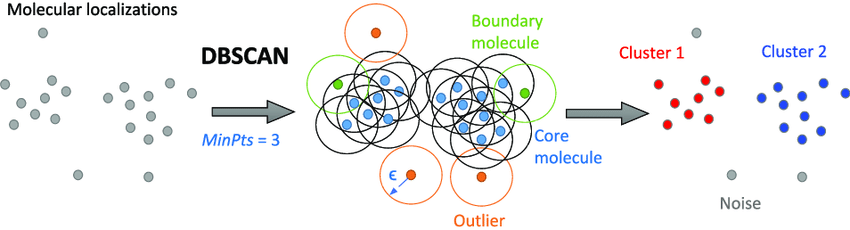
\includegraphics[width=0.9\linewidth]{chapters/clustering/png/An-Example-Illustrating-the-Density-Based-DBSCAN-Clustering-Method-Applied-to-SMLM-Data.png}
    \caption{An Example Illustrating the Density-Based DBSCAN Clustering Method Applied to SMLM Data}
    \label{fig:enter-label-2}
\end{figure}
Возникает 2 параметра: $\varepsilon$ и $m$. Других параметров не будет. От этих параметров и будет зависеть то, какой картина кластеризации получится. Также к преимуществам этого метода относится то, что он не задает заранее количество кластеров, в отличие, например, от k-means, причём количество кластеров будет зависеть от $\varepsilon$ и $m$. 

Как работает алгоритм: берётся произвольная точка, если она имеет плотную окрестность, то дальше рассматривается каждая точка этой плотной окрестности, и вокруг неё также строится $\varepsilon$-окрестность, и так пока не будет достигнута граница некоторого множества объектов. 

Хорошей аналогией может служить лес: один лес - это один кластер, через опушку, второй лес, - другой кластер, мы находимся в лесу. Смотрим, в нашей окрестности деревьев много, это значит, что мы в корневой точке находимся, и дальше мы идём, пока не выйдем на опушку леса, там мы окажемся в граничной точке - она уже не корневая, вокруг деревьев меньше. А где-то могут расти отдельно стоящие деревья - это шумовые выбросы. И вот так ходим по лесу, пока его весь не обойдём, и как только мы обошли весь лес, назовем его кластером. После чего случайно выбираем новое дерево и начинаем строить другой кластер.

Формализуем алгоритм в виде псевдокода:\\
\begin{tabularx}{\linewidth}{lX}
\textbf{вход:} выборка $X^l - \{x_1,...,x_l\}$; параметры $\varepsilon$ и $m$\\
\textbf{выход:} разбиение выборки на кластеры и шумовые выбросы;\\\hspace*{7mm}\hspace*{9mm}$U := X^l$ - не помеченные точки, $a := 0$\\
\textbf{пока} в выборке есть непомеченные точки, $U \neq \emptyset$:\\
\hspace*{7mm} взять случайную точку $x \in U$; \\
\hspace*{7mm} \textbf{если} $\abs{U_\varepsilon (x)} < m$ \textbf{то} \\
\hspace*{7mm}\hspace*{7mm} пометить $x$ как, возможно, шумовой;\\
\hspace*{7mm}\textbf{иначе} \\
\hspace*{7mm}\hspace*{7mm} создать новый кластер: $K:=U_\varepsilon (x); \; a:=a+1;$ \\
\hspace*{7mm}\hspace*{7mm} \textbf{для всех} $x' \in K$, не помеченных или шумовых \\
\hspace*{7mm}\hspace*{7mm}\hspace*{7mm} \textbf{если} $\abs{U_\varepsilon (x')} \geq m$,  \textbf{то} $K := K \cup U_\varepsilon (x')$; \\
\hspace*{7mm}\hspace*{7mm}\hspace*{7mm} \textbf{иначе} поментить $x'$ как граничный кластера $K$;\\
\hspace*{7mm}\hspace*{7mm} $a_j := a$ для всех $x_i \in K$;\\
\hspace*{7mm}\hspace*{7mm} $U := U \backslash K$;\\
\vspace{5mm}
\end{tabularx}

В таком виде алгоритм обладает следующими \textbf{свойствами}:
\begin{itemize}
    \item быстрая кластеризация больших данных: \\$O(l^2)$ в худшем случае, \\ $O(l \mathrm{ln} l)$ при эффективной реализации $U_\varepsilon (x)$;
    \item кластеры произвольной формы
    \item деление объектов на корневые, граничные, шумовые.
\end{itemize}

При этом важно понимать, что граничные объекты не выстраивают в точности границу каждого кластера. Практически это означает, что не стоит всерьез рассматривать граничные объекты, в отличие от шумовых, которые действительно можно в дальнейшем анализировать.

\subsection{Примечание о HDBSCAN} 
От гиперпараметра $\varepsilon$ можно избавиться, используя дивизивную кластеризацию. Такая модификация называется HDBSCAN. Его суть проста: необходимо построить дендрограмму, где по $Oy$ будет отложен $\varepsilon$ (на рис.\ref{fig:hdbdendro} снизу distance). Так мы сможем явно видеть вложенные кластеры. Алгоритм затем сам вычисляет оптимальное количество кластеров на основе метрики "стабильности кластеров".

\begin{figure}[ht!]
    \centering
    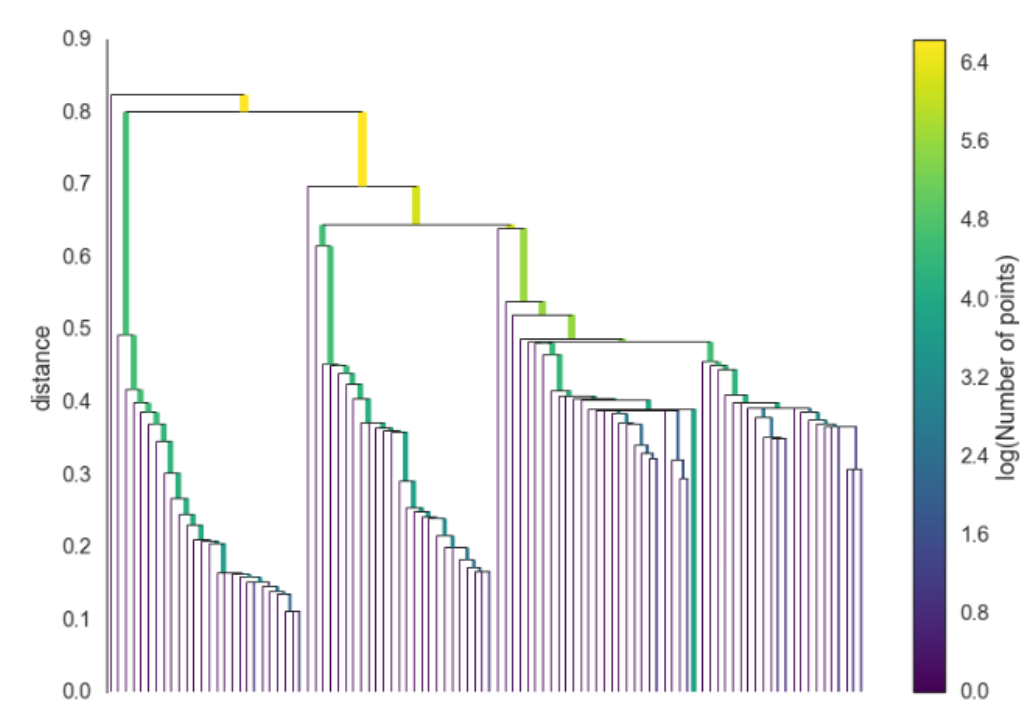
\includegraphics[width=0.6\linewidth]{chapters/clustering/png/hdbscan_dendrogramm.png}
    \caption{К примечанию о HDBSCAN}
    \label{fig:hdbdendro}
\end{figure}
\subsection{Задачи}
\textbf{Задача 1.}

\textbf{Условие.} Применить DBSCAN для выборки из таблицы с $m=4,\;\varepsilon=1.9$. Метрика евклидова.

\begin{center}
\begin{tabular}{ |c|c|c| } 
 \hline
 P1(3,7) & P5(7,3) & P9(3,3) \\ 
 P2(4,6) & P6(6,2) & P10(2,6) \\ 
 P3(5,5) & P7(7,2) & P11(3,5) \\ 
 P4(6,4) & P8(8,4) & P12(2,4) \\ 
 \hline
\end{tabular}
\end{center}

\textbf{Решение.}
Запишем матрицу, составленную из соответственных расстояний между точками выборки:
\begin{center}
\begin{tabular}{ |c|c|c|c|c|c|c|c|c|c|c|c|c|} 
 \hline
dot & P1 & P2 & P3 & P4 & P5 & P6 & P7 & P8 & P9 & P10 & P11 & P12 \\ \hline
P1 & 0 &  &  &  &  &  &  &  &  &  &  &   \\ \hline
P2 & 1.41 & 0 &  &  &  &  &  &  &  &  &  &   \\ \hline
P3 & 2.83 & 1.41 & 0 &  &  &  &  &  &  &  &  &   \\ \hline
P4 & 4.24 & 2.83 & 1.41 & 0 &  &  &  &  &  &  &  &   \\ \hline
P5 & 5.66 & 4.24 & 2.83 & 1.41 & 0 &  &  &  &  &  &  &   \\ \hline
P6 & 5.83 & 4.47 & 3.16 & 2.00 & 1.41 & 0 &  &  &  &  &  &   \\ \hline
P7 & 6.40 & 5.00 & 3.61 & 2.24 & 1.00 & 1.00 & 0 &  &  &  &  &   \\ \hline
P8 & 5.83 & 4.47 & 3.16 & 2.00 & 1.41 & 2.83 & 2.24 & 0 &  &  &  &   \\ \hline
P9 & 4.00 & 3.16 & 2.83 & 3.16 & 4.00 & 3.16 & 4.12 & 5.10 & 0 &  &  &   \\ \hline
P10& 1.41 & 2.00 & 3.16 & 4.47 & 5.83 & 5.83 & 5.66 & 6.40 & 6.32 & 0 &  &   \\ \hline
P11& 2.00 & 1.41 & 2.00 & 3.16 & 4.47 & 4.24 & 5.00 & 5.10 & 2.00 & 1.41 & 0 &   \\ \hline
P12& 2.83 & 3.16 & 4.00 & 5.10 & 4.47 & 5.39 & 6.00 & 1.41 & 2.00 & 2.00 & 1.41 & 0  \\ \hline
\end{tabular}
\end{center}
Сравнивая значения в каждом столбце матрицы с $\varepsilon$ и отбирая те, что меньше этого значения, находим окрестности каждой точки.

\begin{center}
\begin{tabular}{ |c|c| } 
 \hline
 точка & окрестность \\\hline
 P1 & P2, P10\\ 
 P2 & P1, P3, P11\\ 
 P3 & P2, P4\\ 
 P4 & P3, P5\\
 P5 & P4, P6, P7, P8\\
 P6 & P5, P7\\
 P7 & P5, P6\\
 P8 & P5\\
 P9 & P12\\
 P10 & P1, P11\\
 P11 & P2, P10, P12\\
 P12 & P9, P11\\
 \hline
\end{tabular}
\end{center}

Если в окрестности больше $m=4$ точек (включая ее саму), то отнесем эту точку к корневой, иначе - к шумовой.

\begin{center}
\begin{tabular}{ |c|c| } 
 \hline
 точка & тип \\\hline
 P1 & шум\\ 
 P2 & корневая\\ 
 P3 & шум\\ 
 P4 & шум\\
 P5 & корневая\\
 P6 & шум\\
 P7 & шум\\
 P8 & шум\\
 P9 & шум\\
 P10 & шум\\
 P11 & корневая\\
 P12 & шум\\
 \hline
\end{tabular}
\end{center}

Уточним классификацию, учтя граничные точки, т.е. точки, лежащие в окрестности корневых, но при этом не являющимися корневыми:
\begin{center}
\begin{tabular}{ |c|c| } 
 \hline
 точка & тип \\\hline
 P1 & граничная\\ 
 P2 & корневая\\ 
 P3 & граничная\\ 
 P4 & граничная\\
 P5 & корневая\\
 P6 & граничная\\
 P7 & граничная\\
 P8 & граничная\\
 P9 & шум\\
 P10 & граничная\\
 P11 & корневая\\
 P12 & граничная\\
 \hline
\end{tabular}
\end{center}

К первому кластеру отнесем окрестность корневой точки 2, причем в ее окрестности находится еще одна корневая точка 11, так что отнесем и ее окрестность к первому кластеру. Ко второму кластеру отнесем корневую точку 5 и ее окрестность. Осталась лишь одна точка P9, которая не относится ни к какому кластеру и является шумовой.
\begin{figure}[ht!]
    \centering
    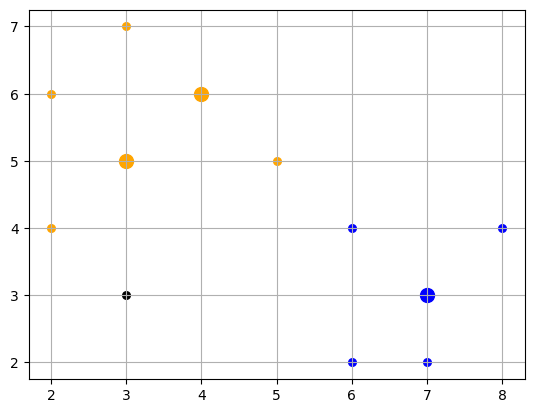
\includegraphics[width=0.7\linewidth]{chapters/clustering/png/task1dbs_plot.png}
    \caption{Кластеризация в задаче 1}
    \label{fig:task1dbs}
\end{figure}

\begin{minipage}{.5\textwidth}
\textbf{Задача 2.}\\
\textbf{Условие.}
  Сравните результаты кластеризации с помощью k-means и с помощью DBSCAN и объясните их.\\
\textbf{Решение.}
Объяснение различий:
\begin{itemize}
\item \textit{Форма кластера}:
K-средние: стремится найти сферические или выпуклые кластеры. Предполагается, что кластеры изотропны (однородны во всех направлениях) и имеют схожий размер.
DBSCAN: может обнаруживать кластеры произвольной формы и размера. Не делает предположений о форме кластеров.
\item \textit{Обработка шума}:
K-средние: плохо справляется с шумом. Точки шума могут быть назначены кластерам, что может повлиять на центры кластеров.
DBSCAN: может идентифицировать и маркировать точки шума, которые не назначены ни одному кластеру.
\end{itemize}
\end{minipage}% This must go next to `\end{minipage}`
\begin{minipage}{.4\textwidth}
      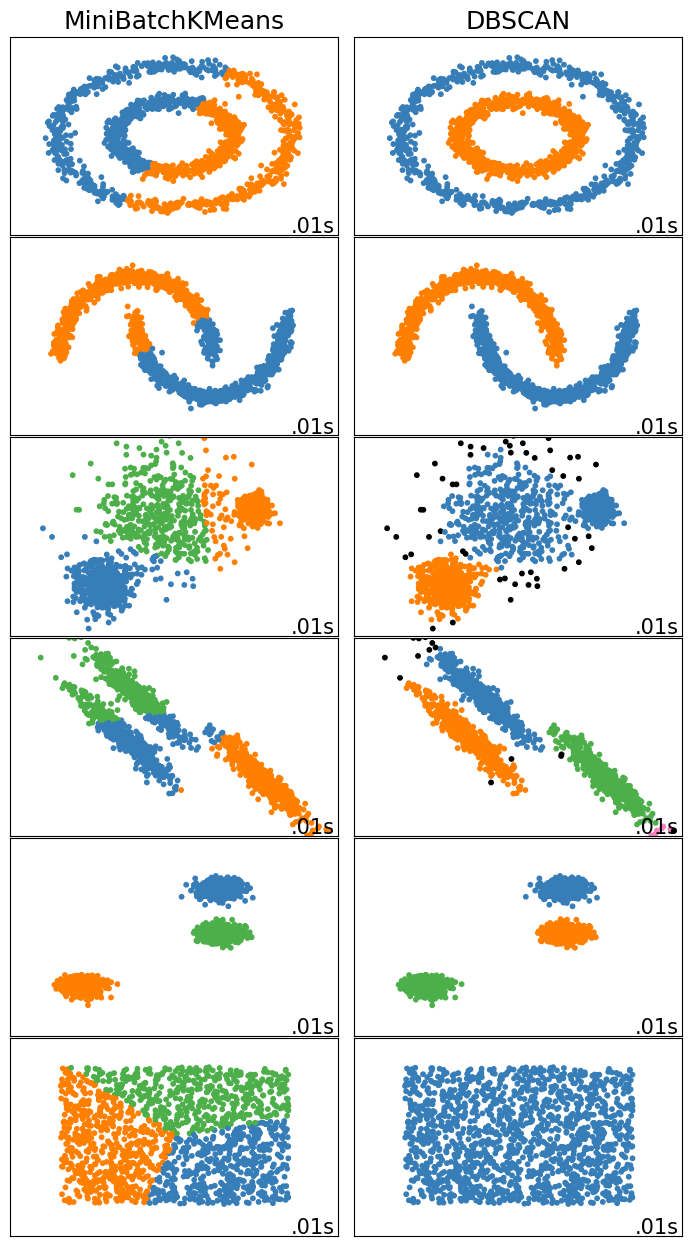
\includegraphics[width=0.95\linewidth]{chapters/clustering/png/task2dbs_plot.png}
\end{minipage}
\begin{itemize}
\item \textit{Плотность кластера}:
K-средние: не учитывает плотность точек. Каждый кластер представлен центроидом.
DBSCAN: учитывает плотность точек. Кластеры формируются на основе плотности точек в окрестности.
\item \textit{Чувствительность параметров}:
K-средние: требует предварительного указания количества кластеров (K), так что, если если заранее указать 3 кластера, то алгоритм и найдет три кластера, даже если он всего один, как на последней паре картинок.
\end{itemize}

\textbf{Задача 3.}\\
\textbf{Предисловие.}
При решении задачи 1 использовалась матрица, состоящая из расстояний между парами точек (\textit{матрица смежности}). Понятием, противоположным расстоянию, является понятие сходства между объектами. Неотрицательная вещественная функция $S(x_i,x_j) = S_{ij}$ называется \textit{мерой сходства}, если:
\begin{itemize}
    \item $0 \leq S(x_i,x_j) < 1$, для $x_i \neq x_j$
    \item $S(x_i,x_j)=1$
    \item $S(x_i,x_j)=S(x_j,x_i)$
\end{itemize}
Пары значений мер сходства можно объединить в \textit{матрицу сходства} $S$, симметричную и единичной диагональю.
\textbf{Условие.}
Применить DBSCAN с пороговым значением \textit{меры сходства} 0.8 и $m = 2$ и заданной матрицей сходства между точками выборки:

\begin{center}
\begin{tabular}{ |c|c|c|c|c|c|} 
 \hline
dot & P1 & P2 & P3 & P4 & P5  \\ \hline
P1 & 1.0 &  &  &  &     \\ \hline
P2 & 0.10 & 1.0 &  &  &  \\ \hline
P3 & 0.41 & 0.64& 1.0 &  & \\ \hline
P4 & 0.55 & 0.47 & 0.44 & 1.0 & \\ \hline
P5 & 0.35 & 0.98 & 0.85 & 0.76 & 1.0 \\ \hline
\end{tabular}
\end{center}

Сравнивая значения в каждом столбце матрицы с $\varepsilon$ и выбирая те точки, для которых значение сходства выше, чем порог, формируем окрестности всех точек.

\begin{center}
\begin{tabular}{ |c|c| } 
 \hline
 точка & окрестность \\\hline
 P1 & -\\ 
 P2 & P5\\ 
 P3 & P5\\ 
 P4 & -\\
 P5 & P2, P3\\
 \hline
\end{tabular}
\end{center}

Если в окрестности больше $m=2$ точек (включая ее саму), то отнесем эту точку к корневой, иначе - к шумовой.

\begin{center}
\begin{tabular}{ |c|c| } 
 \hline
 точка & тип \\\hline
 P1 & шум\\ 
 P2 & корневая\\ 
 P3 & корневая\\ 
 P4 & шум\\
 P5 & корневая\\
 \hline
\end{tabular}
\end{center}

Уточнение классификации, путем учитывания граничных точек, т.е. точек, лежащие в окрестности корневых, но при этом не являющимися корневыми, ничего не дает, т.к. в окрестности точек, определенных как шумовые вообще нет других точек, так что они действительно являются шумом.

К первому кластеру отнесем окрестность корневой точки P2, причем в ее окрестности находятся еще краевая точка P5, так что отнесем ее к этому же кластеру. В окрестности точки P5 помимо уже классифицированной P2 находится еще корневая точка P3, которую также отнесем к первому кластеру. Остальные точки классифицированы как шумовые. Таким образом в данной задаче всего один кластер, состоящий из точек P2, P3, P5.

\section{Агломеративная иерархическая кластеризация}
Иерархические алгоритмы кластеризации, также известные как алгоритмы таксономии, создают не одно, а несколько вложенных разбиений выборки на непересекающиеся классы. Результаты такой кластеризации обычно визуализируются в форме дендрограммы — дерева, которое иллюстрирует структуру кластеров и их взаимосвязи. Классическим примером может служить иерархическая классификация живых организмов, таких как животные и растения. \\
Среди алгоритмов иерархической кластеризации выделяются два основных типа. Дивизивные или нисходящие алгоритмы начинают с одного общего кластера и последовательно разбивают его на более мелкие подмножества. В отличие от них, агломеративные или восходящие алгоритмы работают по принципу объединения объектов в всё более крупные кластеры, начиная с того, что каждый объект представляет собой отдельный кластер.


\subsection{Описание алгоритма}
\begin{enumerate}
    \item Инициализировать множество кластеров $C_1$:  
    \[
    t := 1; \quad C_t = \{\{x_1\}, \{x_2\}, \ldots, \{x_\ell\}\}.
    \]
    \item Для всех $t = 2, \ldots, \ell$ (где $t$ — номер итерации):
    \begin{enumerate}
        \item Найти в $C_{t-1}$ два ближайших кластера $U, V$ и вычислить расстояние между ними $R(U, V)$:
        \[
        (U, V) := \arg \min_{U \neq V} R(U, V);
        \]
        \[
        R_t := R(U, V).
        \]
        \item Изъять кластеры $U$ и $V$, добавить объединённый кластер $W = U \cup V$:
        \[
        C_t := C_{t-1} \cup \{W\} \setminus \{U, V\}.
        \]
        \item Для всех $S \in C_t$ вычислить R(W, S) по формуле Ланса-Уильямса:
        \[
R(W, S) = \alpha_U R(U, S) + \alpha_V R(V, S) + \beta R(U, V) + \gamma |R(U, S) - R(V, S)|
        \]
    \end{enumerate}
\end{enumerate}

\subsection{Описание алгоритма для частичного обучения}
Если даны размеченные объекты $\{x_1, x_2, \ldots, x_k\}$, то алгоритм будет уже выглядеть по-другому:
\begin{enumerate}
    \item Инициализировать множество кластеров $C_1$:  
    \[
    t := 1; \quad C_t = \{\{x_1\}, \{x_2\}, \ldots, \{x_\ell\}\}.
    \]
    \item Для всех $t = 2, \ldots, \ell$ (где $t$ — номер итерации):
    \begin{enumerate}
        \item Найти в $C_{t-1}$ два ближайших кластера $U, V$ и вычислить расстояние между ними $R(U, V)$, \textbf{при условии, что в $U \cup V$ нет объектов с разными метками}:
        \[
        (U, V) := \arg \min_{U \neq V} R(U, V);
        \]
        \[
        R_t := R(U, V).
        \]
        \item Изъять кластеры $U$ и $V$, добавить объединённый кластер $W = U \cup V$:
        \[
        C_t := C_{t-1} \cup \{W\} \setminus \{U, V\}.
        \]
        \item Для всех $S \in C_t$ вычислить R(W, S) по формуле Ланса-Уильямса:
        \[
R(W, S) = \alpha_U R(U, S) + \alpha_V R(V, S) + \beta R(U, V) + \gamma |R(U, S) - R(V, S)|
        \]
    \end{enumerate}
\end{enumerate}

\subsection{Построение дендрограммы}
Дендрограммы графически иллюстрируют иерархическую кластеризацию. По горизонтали располагаются кластеры, а по вертикали — расстояния \( R_t \). 

При построении дендрограммы важно учитывать, что линии не должны нигде пересекаться. 

Определение числа кластеров наиболее удобно осуществлять путем отсечения правой части дендрограммы. На горизонтальной оси находится интервал максимальной длины \( |R_{t+1} - R_t| \).

Количество кластеров определяется по формуле:
\[
K = \ell - t + 1,
\]
где \( \ell \) — общее количество итераций.

Ниже представлен пример  дендрограммы:

\begin{figure}[h!]
    \centering
    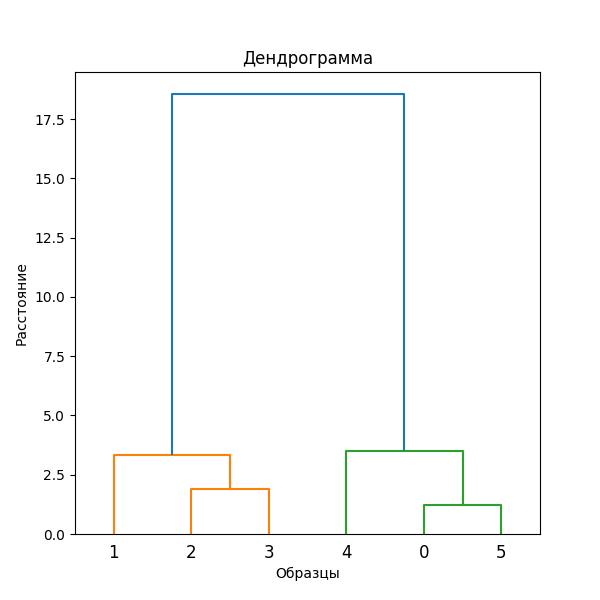
\includegraphics[width=0.2\textwidth]{png/example.jpg} % Укажите путь к картинке
    \caption{Пример дендрограммы}
\end{figure}


\subsection{Частные случаи формулы Ланса-Уильямса}

На практике используются следующие способы вычисления расстояний \( R(W, S) \) между кластерами \( W \) и \( S \).

\textbf{1. Расстояние ближнего соседа}
\[
R_b(W, S) = \min_{w \in W, s \in S} \rho(w, s),
\]
где \( \alpha_U = \alpha_V = \frac{1}{2}, \beta = 0, \gamma = -\frac{1}{2} \).

\textbf{2. Расстояние дальнего соседа}
\[
R_d(W, S) = \max_{w \in W, s \in S} \rho(w, s),
\]
где \( \alpha_U = \alpha_V = \frac{1}{2}, \beta = 0, \gamma = \frac{1}{2} \).

\textbf{3. Среднее расстояние}
\[
R_c(W, S) = \frac{1}{|W||S|} \sum_{w \in W} \sum_{s \in S} \rho(w, s),
\]
где \( \alpha_U = \frac{|U|}{|W|}, \alpha_V = \frac{|V|}{|W|}, \beta = 0, \gamma = 0 \).

\textbf{4. Расстояние между центрами}
\[
R_c(W, S) = \rho^2\left(\frac{\sum_{w \in W} w}{|W|}, \frac{\sum_{s \in S} s}{|S|}\right),
\]
где \( \alpha_U = \frac{|U|}{|W|}, \alpha_V = \frac{|V|}{|W|}, \beta = -\alpha_U\alpha_V, \gamma = 0 \).

\textbf{5. Расстояние Уорда}
\[
R_u(W, S) = |S||W|\frac{\rho^2\left(\frac{\sum_{w \in W} w}{|W|}, \frac{\sum_{s \in S} s}{|S|}\right)}{|S| + |W|},
\]
где \( \alpha_U = \frac{|S| + |U|}{|S| + |W|},\,  \alpha_V =  \frac{|S| + |V|}{|S| + |W|},\,  \beta = -\frac{|S|}{|S| + |W|},\,  \gamma = 0. \)

\subsection{Свойства иерархической кластеризации}

\begin{itemize}

    \item \textbf{Сжатие}:
    \[
R_t \leq \rho(\mu_U, \mu_V), \quad \forall t.
\]
    \item \textbf{Растяжение}:
    \[
R_t \ge \rho(\mu_U, \mu_V), \quad \forall t.
\]
    \item \textbf{Монотонность}: Дендрограмма не имеет самопересечений, при каждом слиянии расстояние между объединяемыми кластерами только увеличивается

    Оказывается, не любое сочетание коэффициентов в формуле Ланса-Вильямса приводит к монотонной кластеризации. \\
    \textbf{Теорема Миллигана} \\
    Если выполняются следующие три условия, то кластеризация является монотонной:

\begin{enumerate}
    \item \( \alpha_U > 0, \quad \alpha_V > 0; \)
    \item \( \alpha_U + \alpha_V + \beta > 1; \)
    \item  \( \min\{\alpha_U, \alpha_V\} + \gamma > 0. \)
\end{enumerate}
\end{itemize}

Из перечисленных выше расстояний только \( R_c \) не является монотонным. 

\subsection{Задачи}
\textbf{Задача 1.}
Даны точки:
\[
X = \{(1, 2), (1, 4), (2, 3), (8, 8), (8, 9)\}.
\]
Необходимо провести агломеративную иерархическую кластеризацию с использованием метода дальнего соседа и построить дендрограмму.

Примечание: Используем метрику Евклида для вычисления расстояний между точками

\textbf{Решение}
\[
d((x_1, y_1), (x_2, y_2)) = \sqrt{(x_1 - x_2)^2 + (y_1 - y_2)^2}.
\]

\begin{itemize}
    \item \( d((1, 2), (1, 4)) = 2 \)
    \item \( d((1, 2), (2, 3)) \approx 1.41 \)
    \item \( d((1, 2), (8, 8)) \approx 9.22 \)
    \item \( d((1, 2), (8, 9)) \approx 9.90 \)
    \item \( d((1, 4), (2, 3)) \approx 1.41 \)
    \item \( d((1, 4), (8, 8)) \approx 8.06 \)
    \item \( d((1, 4), (8, 9)) \approx 8.60 \)
    \item \( d((2, 3), (8, 8)) \approx 7.81 \)
    \item \( d((2, 3), (8, 9)) \approx 8.49 \)
    \item \( d((8, 8), (8, 9)) = 1 \)
\end{itemize}

На первом шаге находим пару точек с минимальным расстоянием: \( (8, 8) \) и \( (8, 9) \), с расстоянием 1. Объединяем их в кластер \( C_1 = \{(8, 8), (8, 9)\} \).

Теперь пересчитываем расстояния между новым кластером и остальными точками:
\begin{itemize}
    \item \( d(C_1, (1, 2)) = \max(d((8, 8), (1, 2)), d((8, 9), (1, 2))) \approx 9.90 \)
    \item \( d(C_1, (1, 4)) = \max(d((8, 8), (1, 4)), d((8, 9), (1, 4))) \approx 8.60 \)
    \item \( d(C_1, (2, 3)) = \max(d((8, 8), (2, 3)), d((8, 9), (2, 3))) \approx 8.49 \)
\end{itemize}

Теперь выбираем пару с минимальным расстоянием: \( (1, 2) \) и \( (2, 3) \), с расстоянием \( \sqrt{2} \approx 1.41 \). Объединяем их в кластер \( C_2 = \{(1, 2), (2, 3)\} \).

Теперь пересчитываем расстояния между этим кластером и остальными:
\begin{itemize}
    \item \( d(C_2, (1, 4)) = \max(d((1, 2), (1, 4)), d((2, 3), (1, 4))) = 2 \)
    \item \( d(C_2, C_1) = \max(d((1, 2), (8, 8)), d((1, 2), (8, 9)), d((2, 3), (8, 8)), d((2, 3), (8, 9))) = 9.90 \)
\end{itemize}

Теперь объединяем \( C_2 = \{(1, 2), (2, 3)\} \) и \( (1, 4) \), так как их расстояние равно 2.

Теперь у нас есть два кластера:
\[
C_3 = \{(1, 2), (2, 3), (1, 4)\}, \quad C_1 = \{(8, 8), (8, 9)\}.
\]

Наконец, объединяем два оставшихся кластера \( C_3 \) и \( C_1 \), так как расстояние между ними равно 9.90.

\begin{figure}[h!]
    \centering
    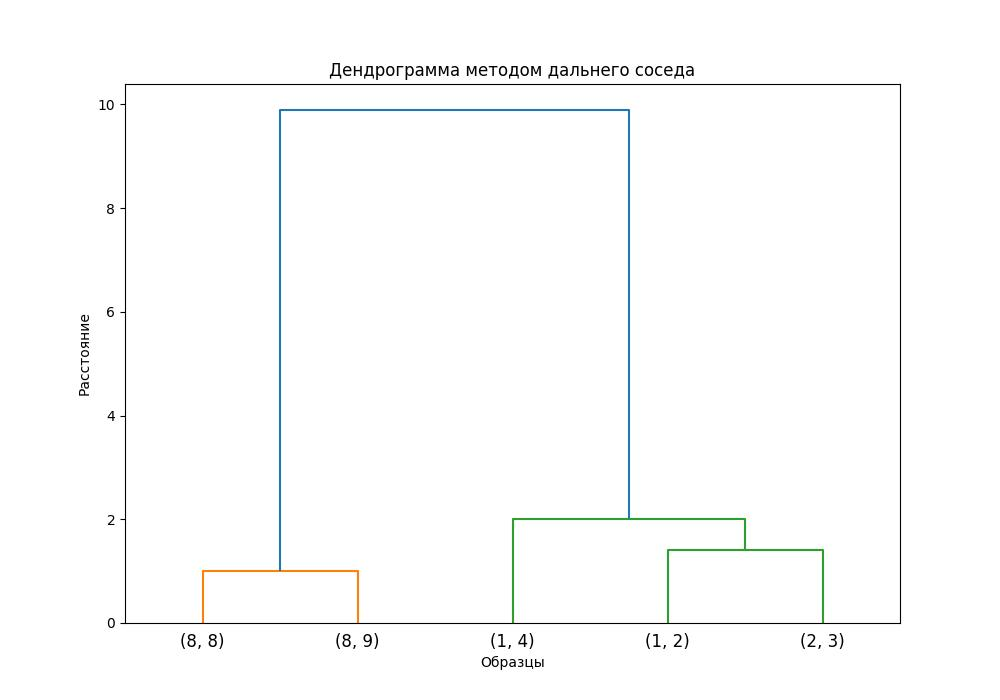
\includegraphics[width=0.5\textwidth]{png/figure1.jpg} % Укажите путь к картинке
    \caption{Дендрограмма методом дальнего соседа}
\end{figure}


\textbf{Задача 2.} Доказать, что расстояние между центрами не является монотонным
\textbf{Доказательство.}
Формула Ланса-Уильямса при вычислении расстояния между центрами: 
$R_{\text{ц}}(W, S) = \rho^2 \left( \sum_{w \in W} w \frac{1}{|W|} , \sum_{s \in S} s \frac{1}{|S|} \right)$
\[
\alpha_U = \frac{|U|}{2}, \quad \alpha_V = \frac{|V|}{2}, \quad \beta = -\alpha_U \cdot \alpha_V, \quad \gamma = 0.
\]

Теорема Миллигана утверждает, что кластеризация является монотонной, если выполняются следующие три условия для параметров \( \alpha_U \), \( \alpha_V \) и \( \beta \):

\begin{enumerate}
    \item \( \alpha_U \geq 0 \), \( \alpha_V \geq 0 \)
    \item \( \alpha_U + \alpha_V + \beta \geq 1 \)
    \item \( \min(\alpha_U, \alpha_V) + \gamma \geq 0 \)
\end{enumerate}

Рассмотрим первую итерацию, когда $|U|=1$, $|V|=1$, а значит $|W|=2$.

Тогда:
\[
\alpha_U = \frac{1}{2}, \quad \alpha_V = \frac{1}{2}, \quad \beta = -\frac{1}{2} \cdot \frac{1}{2}.
\]

Рассмотрим условие 2 теоремы Миллигана:

\[
\alpha_U + \alpha_V + \beta = \frac{1}{2} + \frac{1}{2} - \left( \frac{1}{2} \cdot \frac{1}{2} \right)=1 - \frac{1}{4} = \frac{3}{4}.
\]

Это значение меньше 1, следовательно, второе условие не выполняется, и теорема Миллигана не выполняется для метода центроидного расстояния.

\textbf{Задача 3.}
По данной дендрограмме определить количество кластеров, пояснить свой выбор.

\begin{figure}[h!]
    \centering
    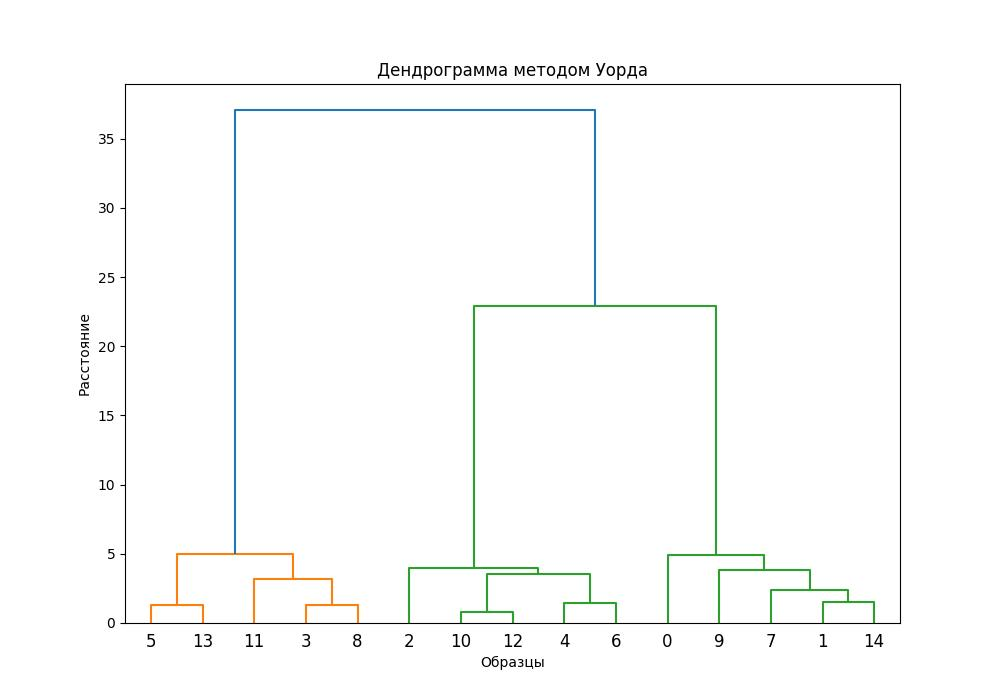
\includegraphics[width=0.5\textwidth]{png/figure2.jpg} % Укажите путь к картинке
    \caption{Дендрограмма методом Уорда}
\end{figure}

\textbf{Решение.}

Для нахождения числа кластеровмы ищем интервал максимальной длины \( |R_{t+1} - R_t| \), где \( R_t \) и \( R_{t+1} \) — расстояния между кластерами на каждом шаге слияния. На основе этих интервалов и максимального изменения расстояний между слияниями можно определить точку \( t \).
Количество кластеров находится по формуле: 
$K=l - t - 1$, где l - количество итераций

В нашем случае t = 12, l = 14, значит K = 14-12+1 = 3

\textbf{Ответ.} 3

\section{Простые эвристические методы частичного обучения}
\subsection{Постановка задачи}
Существует привычная нам задача классификации. Мы имеем $X$ --- множество объектов с известными признаками и $Y$ --- пространство классов. Есть неизвестная функция $X \longrightarrow Y$, сопоставляющая каждому обьекту его класс. Имеется обучающая выборка $\{x_1, x_2, ...\} \subset X$ и соответствующие им известные классы $\{y_1, y_2, ...\} \subset Y$. Задача классификации сводится к построению классификатора --- некой аппроксимации неизвестной функции $X \longrightarrow Y$. \\

С другой стороны существует задача кластеризации. Мы все также имеем $X$ --- множество объектов. И хотим аппроксимировать функцию $X \longrightarrow Y$. Но на этот раз у нас нет обучающей выборки, зато есть функция расстояния между объектами $\rho: X\times X \longrightarrow \mathbb{R}$. И в этом случае кластеризующая функция строится не на основе обучающей выборки, а так чтобы расстояние между объектами одного кластера было мало, а расстояние между объектами разных кластеров было велико. \\

Первый случай называется обучение с учителем,а кластеризация называется обучением без учителя. Где-то по середине между этими задачами находится задача частичного обучения. В этом случае у нас все также есть множество обьектов из $X$ и (возможно) функция $\rho$. При этом только для некоторой доли имеющихся обьектов известна классовая принадлежность. Иначе говоря обучающая выборка размечена \textbf{частично}. \\

Приведем пример (Рис. 1). Допустим известные обьекты в пространстве признаков имеют вид в виде двух бананов. И нам известна принадлежность только двух точек. В таком случае чистая задача кластеризации обучит классификатор только по двум точкам, который будет иметь сомнительное качество на всех остальных данных. При это частичное обучение могло бы учесть явную кластеризацию данных и дать значительно лучшую классификацию.\\

\begin{center}
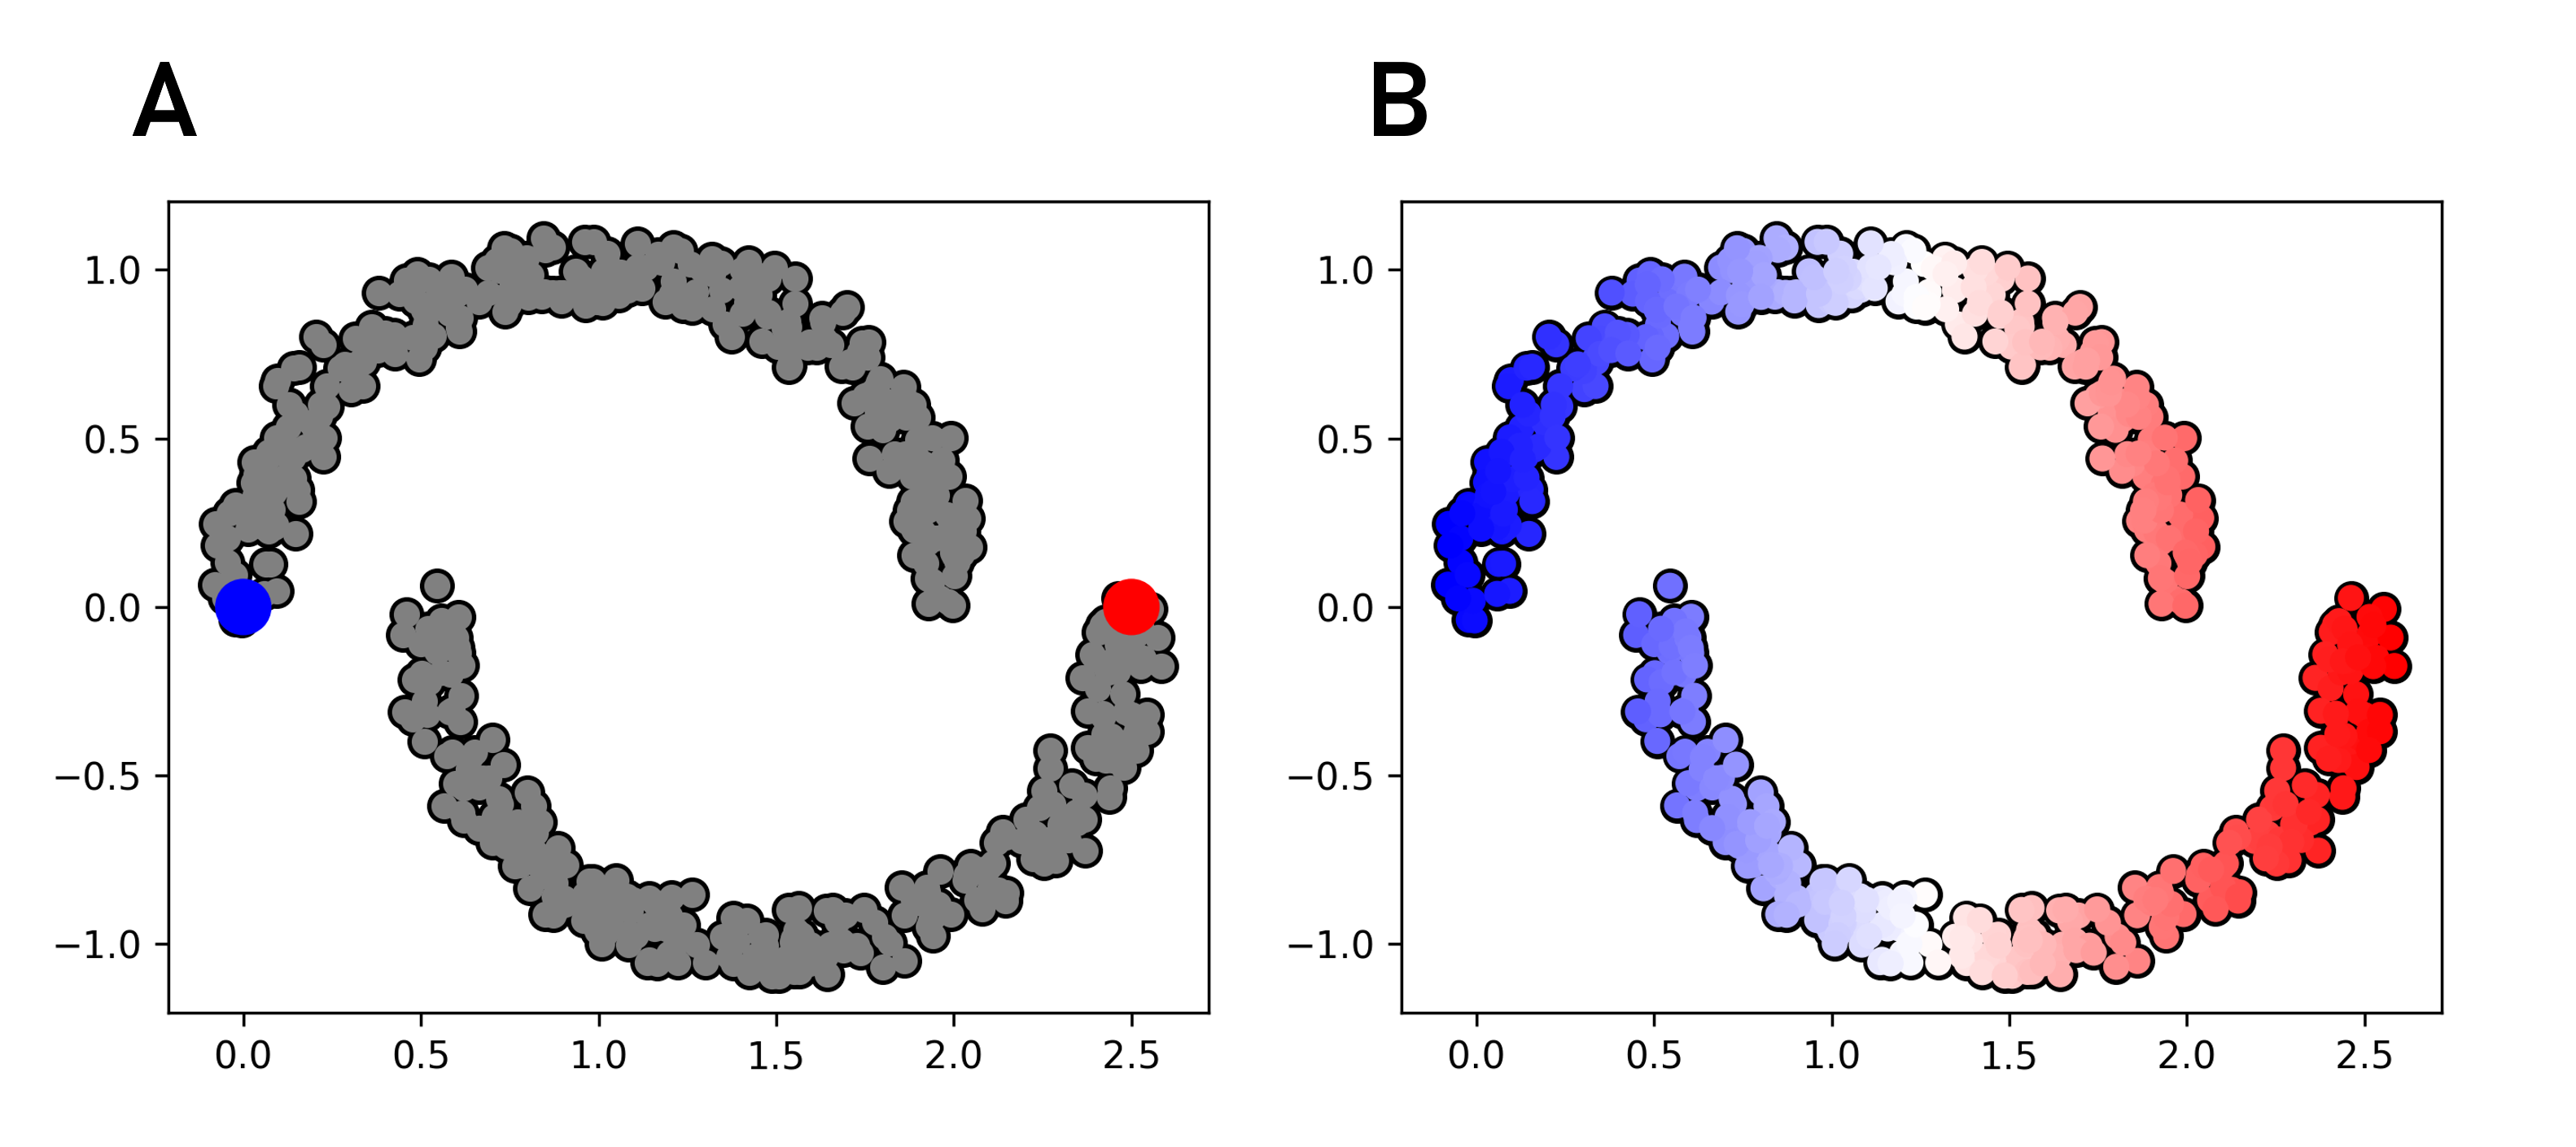
\includegraphics[width=1.0\textwidth]{chapters/clustering/picture_1.png}
\textbf{Рисунок 1.} (\textbf{A}) Пример частично размеченных данных. (\textbf{B}) Классификация обученная на размеченных данных не учитывает кластерную структуру неразмеченных. 
\end{center}

Однако частичное обучение не может сводиться только к кластеризации, представьте теперь, что мы знаем классы уже трех точек на выборке из двух бананов (Рис. 2). В таком случае кластеризация дала бы предсказание которое не может соотноситься с известными классами всех трех точек. Таким образом задача частичного обучения действительно находится посередине между классификацией и кластеризацией, но не является ни тем, ни другим. \\
\begin{center}
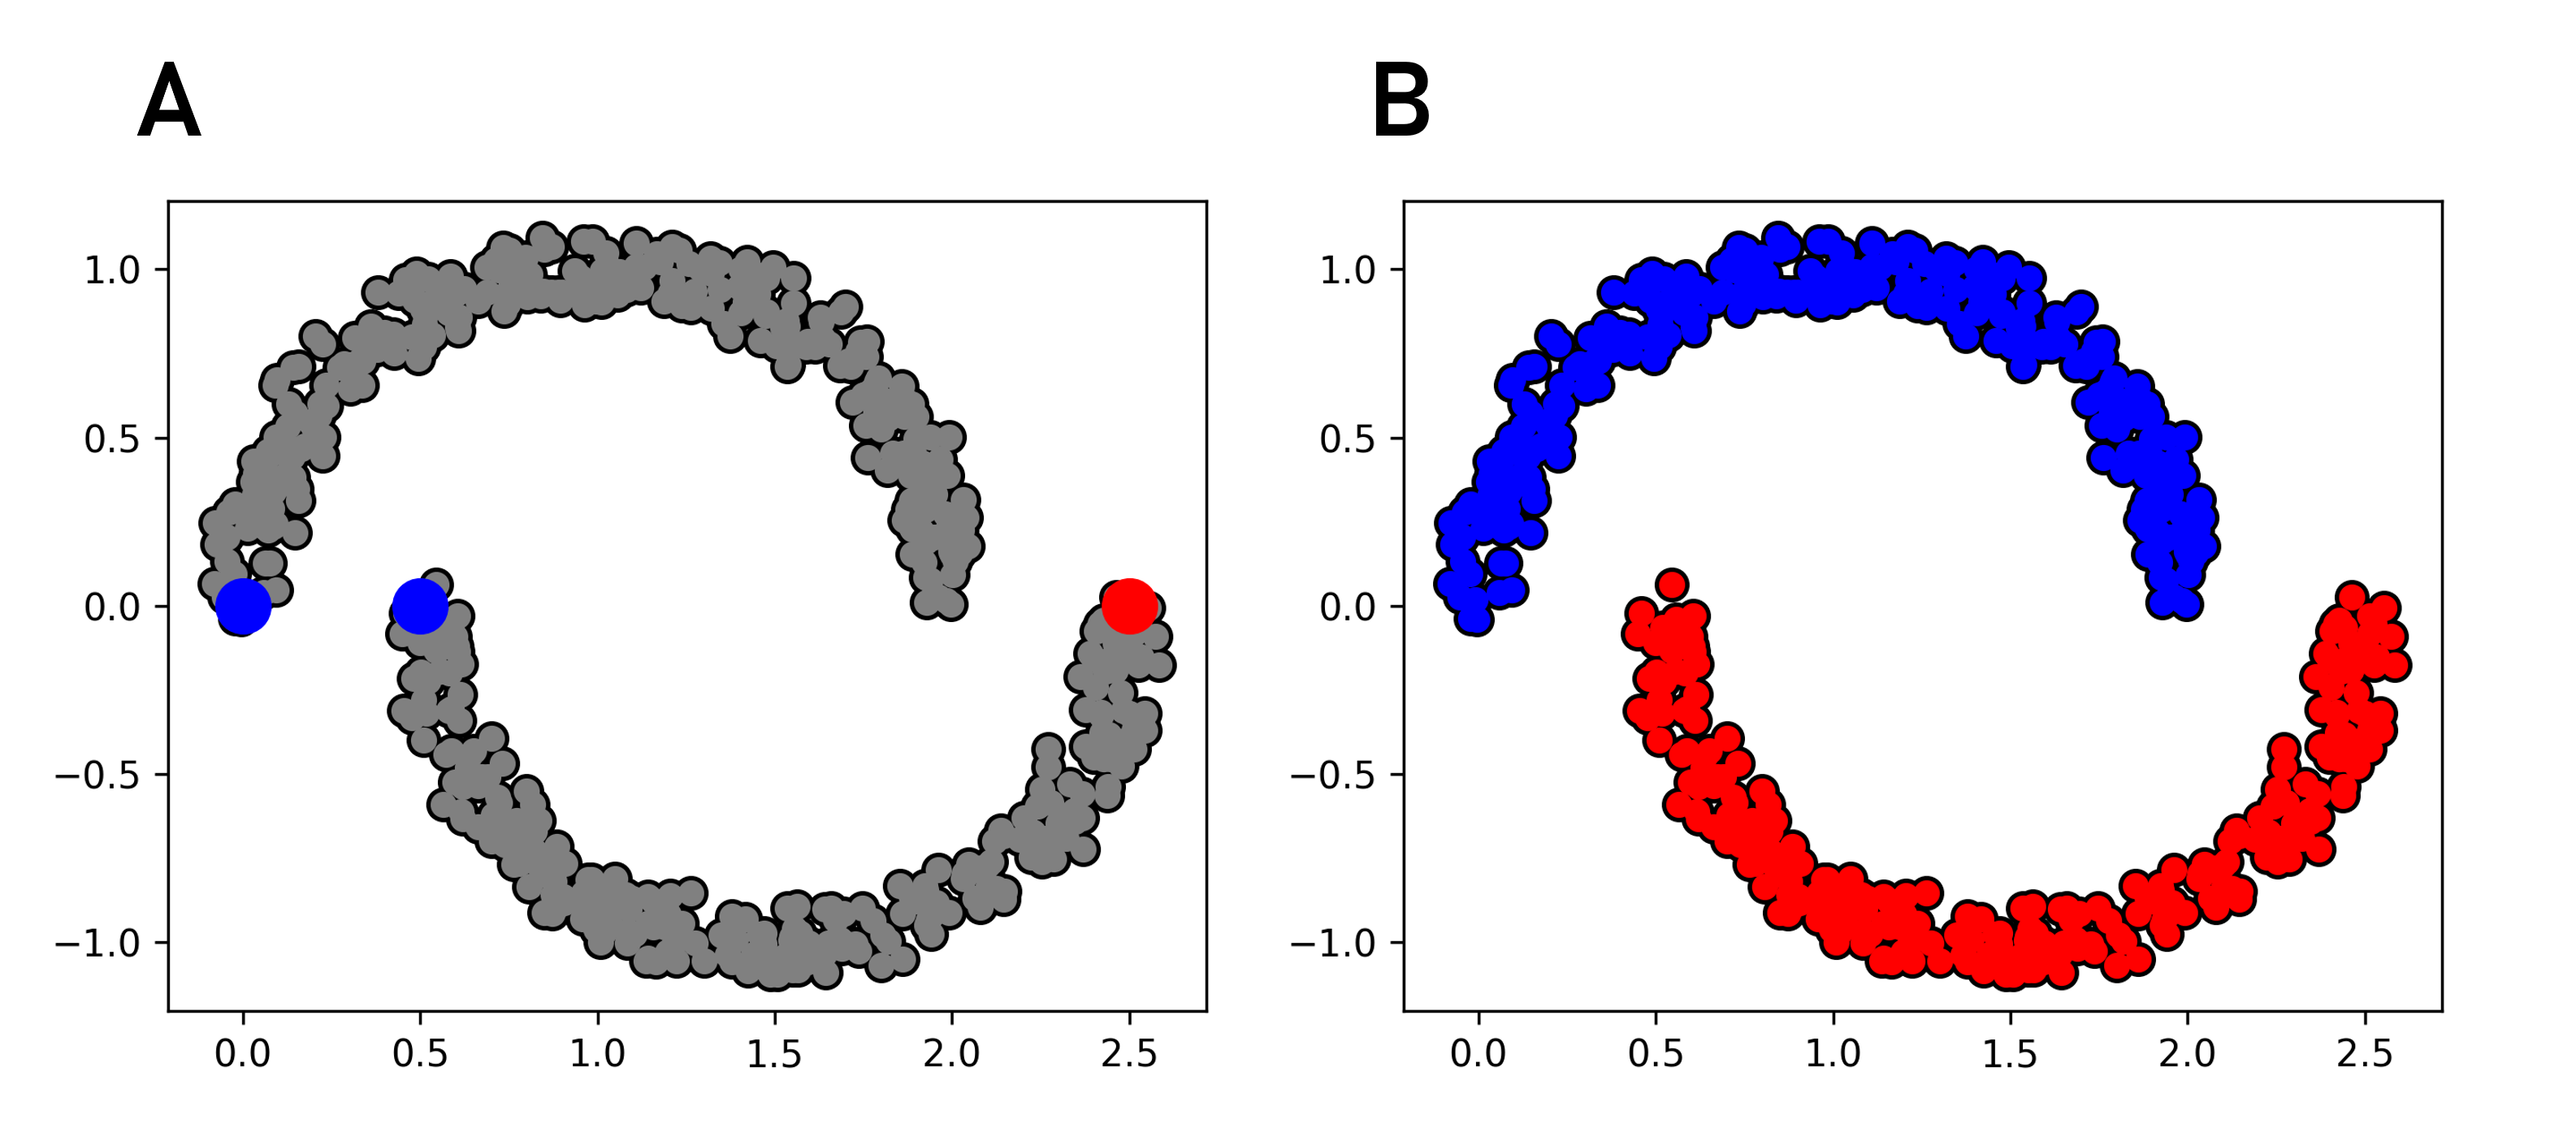
\includegraphics[width=1.0\textwidth]{chapters/clustering/picture_2.png}
\textbf{Рисунок 2.} (\textbf{A}) Пример частично размеченных данных. (\textbf{B}) Кластеризация не учитывает классовую принадлежность размеченных данных. 
\end{center}

Приведем пример: программист решил сделать классификатор для фотографий котиков и собачек, для этого он скачал по миллиону фотографий и тех и других. Однако, ему хватило сил подписать котик это или собачка только для 1000 фотографий. Классификация не может быть построена только по 1000 фотографиям --- мало данных, а кластеризация может разбить фотографии неизвестным образом --- по цвету фона, по размеру животного. И только частичное обучение может помочь ленивому программисту.
\subsection{Self-training}
Каким же образом можно реализовать частичное обучение? Рассмотрим подход, который называется self-training (само-обучение). Вернемся к датасету с бананами в котором известны классы двух точек. Как было сказано ранее построение классификатора по двум точкам тут не поможет. Однако допустим, что мы все же построили классификатор по двум точкам, к примеру логистическую регрессию. Вспомним что многие методы классификации могут оценивать свою уверенность в предсказании. Тогда для некоторых точек с наибольшей уверенностью классификации (скажем 5\% самых уверенных) предсказание  классификации может оказаться вполне верным. Давайте же дополним обучающую выборку классификатора этими точками. На второй итерации нашего подхода мы обучим классификатор уже по дополненной обучающей выборке. Выполнив предсказание для остальных данных, выберем еще раз 5\% ранее неразмеченных точек с наибольшей уверенностью и пополним ими обучающую выборку. Будем повторять такие итерации пока не классифицируем все точки в нашем датасета. Как мы видим, результат такого подхода заметно лучше, чем у классификации по двум исходным точкам. 
\begin{center}
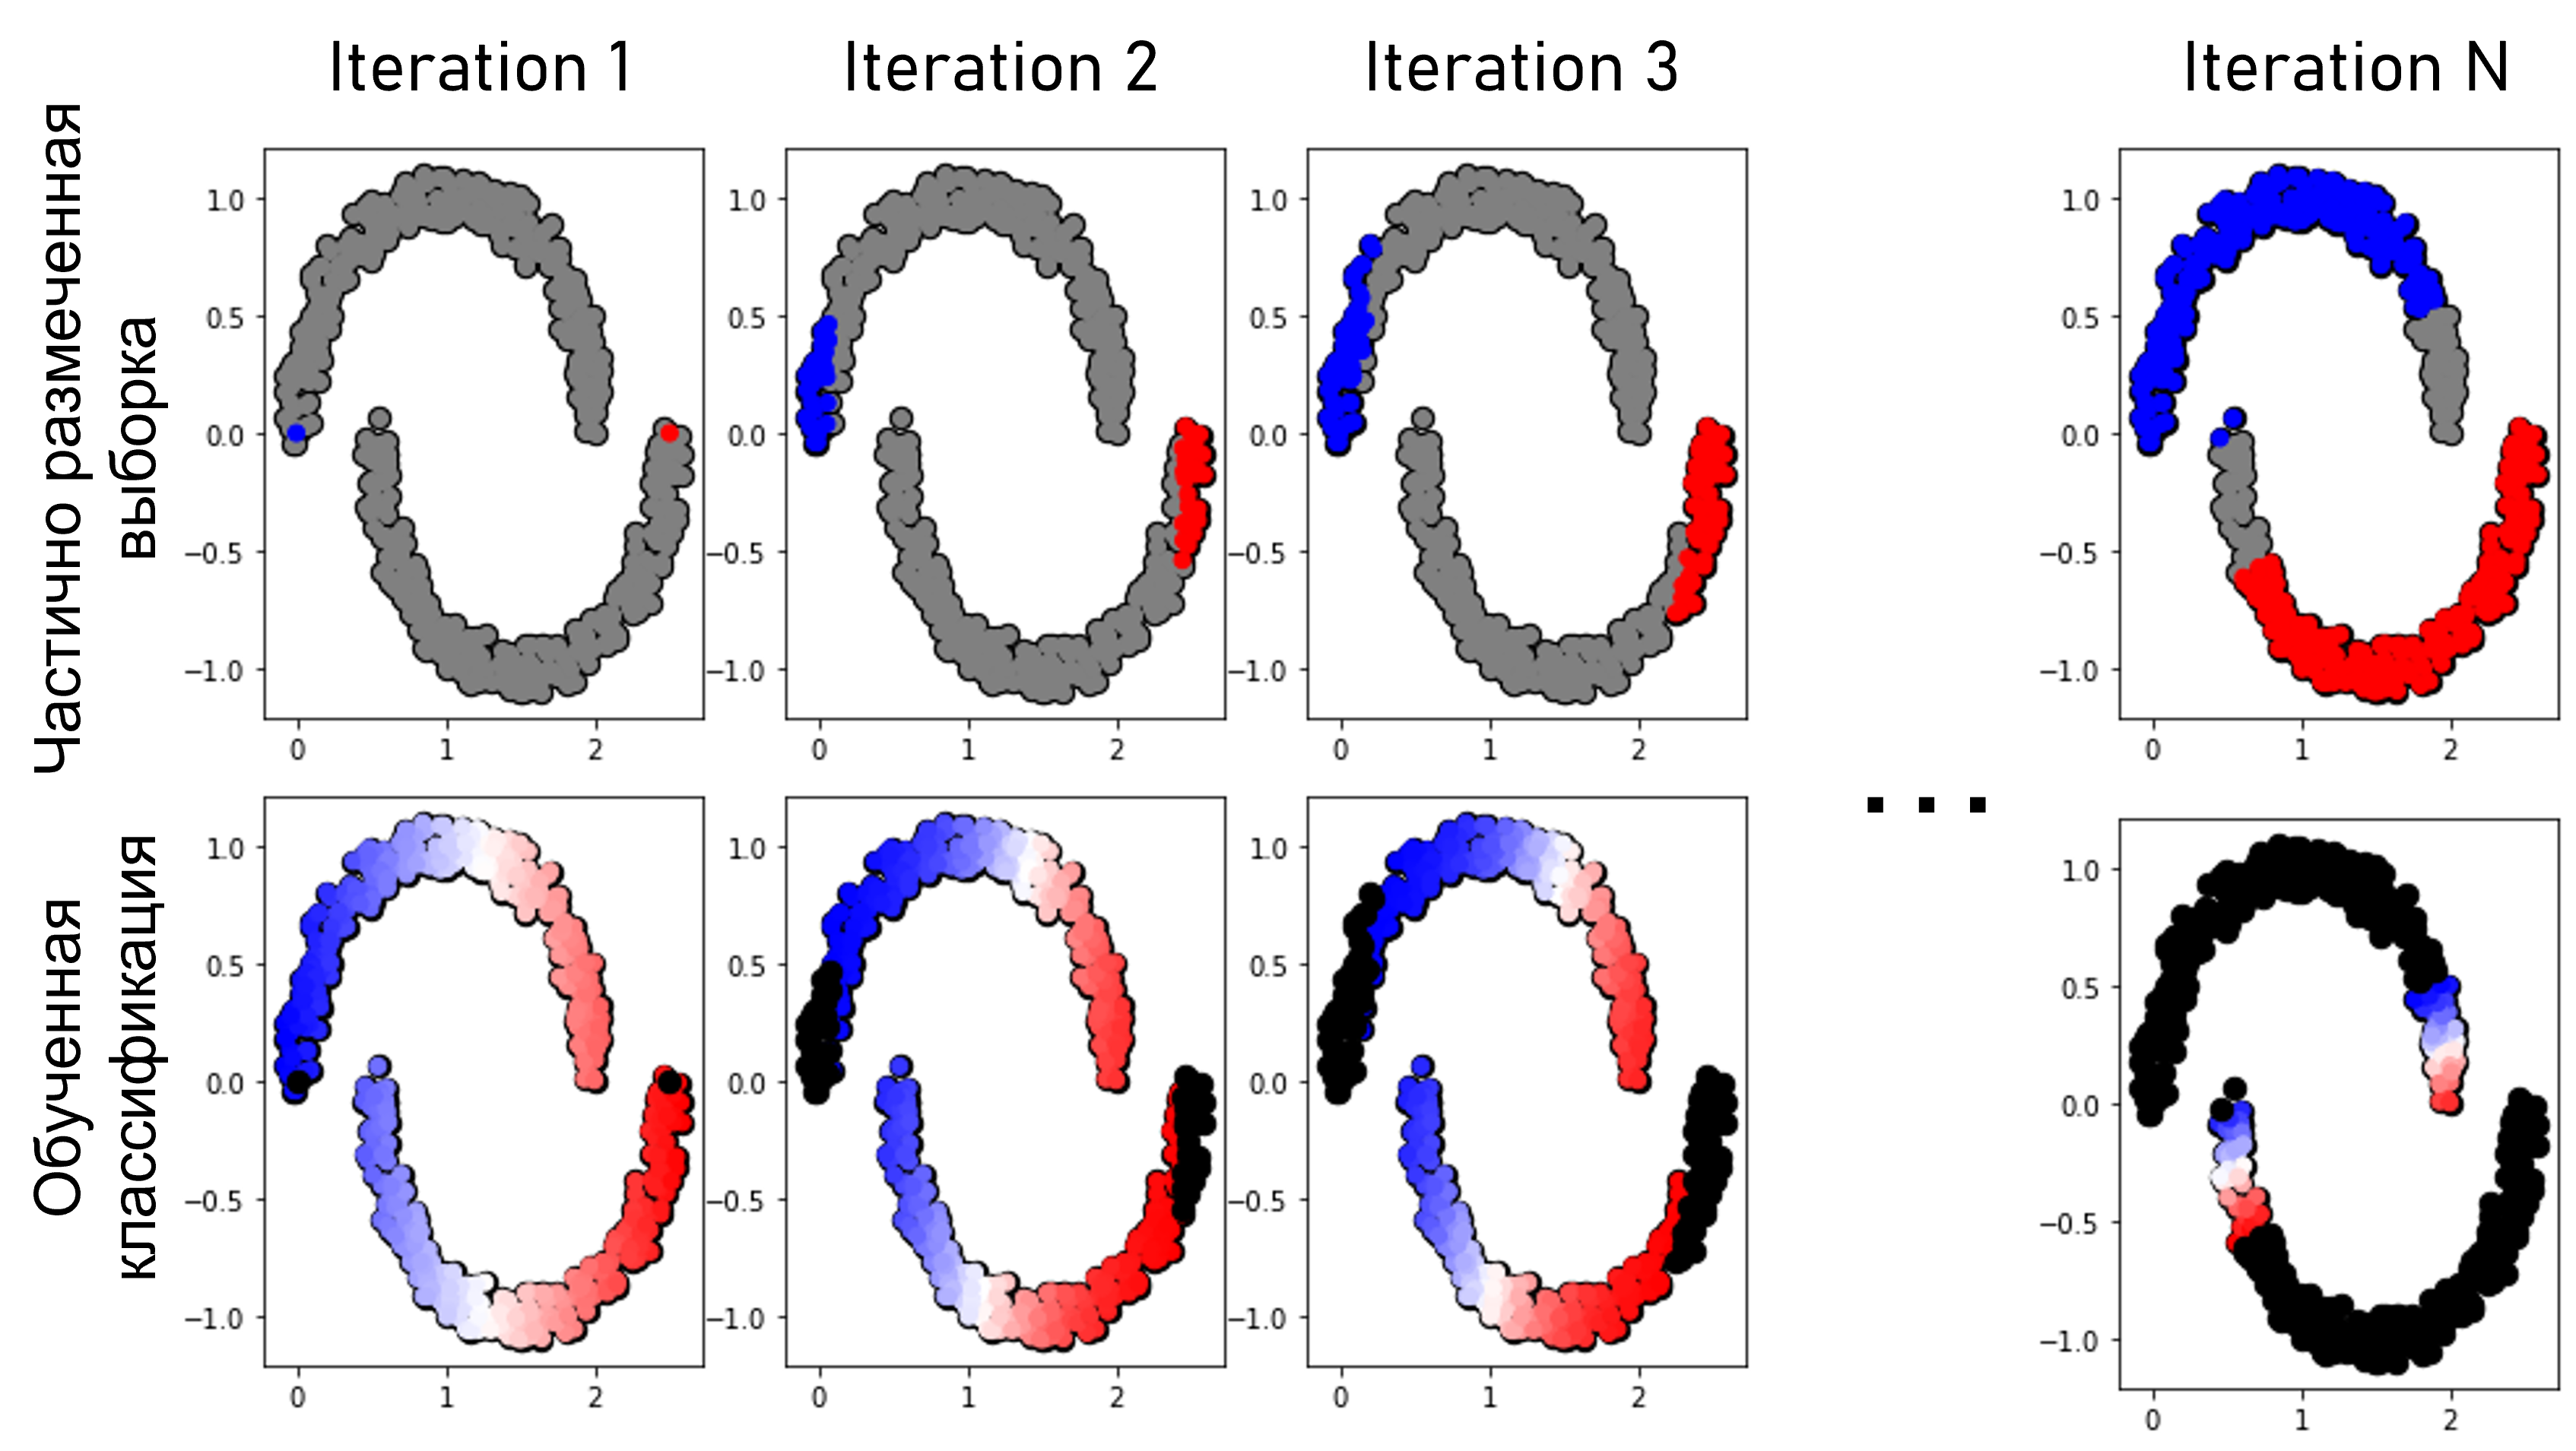
\includegraphics[width=1.0\textwidth]{chapters/clustering/picture_3.png}
\textbf{Рисунок 3.} Пример работы итераций self-training. 
\end{center}
Оформим описанный процесс более математизировано. Пусть мы строим функцию $a: X \longrightarrow Y$. Пусть у нас есть метод обучения функции $\mu: Z \longrightarrow a$ который принимает на вход размеченную часть выборки $Z \subset X$. Допустим функция $a$ имеет вид
\begin{equation*}
    a(x) = \arg \max_{y \subset Y}\Gamma_y(x)
\end{equation*}
где $\Gamma_y(x)$ это некоторые (к примеру) линейные функции от $x \subset X$ которые обучаются так, чтобы быть большими, если $x$ принадлежит классу $y$ и маленькими в противном случае. В таком случае уверенность классификации в принадлежности элемента $x$ к классу $y_1$ (отступ):
\begin{equation*}
    M_1(x) = \Gamma(x) - \max_{y \subset Y\backslash y_1}\Gamma_{y_1}(x) 
\end{equation*}
Пусть $Z$ это размеченная часть обучающей выборки. Тогда алгоритм выглядит так:
\begin{enumerate}
  \item $a = \mu(Z)$ --- обучить классификатор на размеченной выборке
  \item $\Delta := \{x \subset X\backslash Z \;|\; M(x) \geq M_0 \}$ --- выбрать несколько точек из неразмеченной части выборки которые наиболее уверенно классифицируются. 
  \item $Z := Z\cup\Delta$ --- дополнить размеченную выборку
  \item Если не все элементы выборки размечены, вернуться в начало.
\end{enumerate}
\subsection{Сo-training}
Рассмотрим более узкий кейс, допустим у нас есть не один, а целых два метода обучения классификации $\mu_1, \mu_2$, которые принципиально отличаются друг от друга, например имеют разные парадигмы обучения, и/или используют разные признаки обьектов, и/или имеют разную стартовую выборку. В таком случае мы можем получить преимущество в частичном обучении заставив их учить друг друга по следующему алгоритму:
\begin{enumerate}
  \item $a_1 = \mu_1(Z_1)$\\
  $a_2 = \mu_2(Z_2)$ --- два метода обучают классификаторы на своих размеченных выборках. 
  \item $\Delta_1 := \{x \subset X\backslash Z_1\backslash Z_2 \;|\; M_1(x) \geq M_{01} \}$ --- метод 1 размечает неразмеченные точки, в которых он уверен.\\
  $\Delta_2 := \{x \subset X\backslash Z_1\backslash Z_2 \;|\; M_2(x) \geq M_{02} \}$ --- метод 2 делает тоже самое.
  \item $Z_1 := Z_1\cup\Delta_2$ --- метод 2 дополняет обучающую выборку метода 1 \\
  $Z_2 := Z_2\cup\Delta_1$ --- метод 1 дополняет обучающую выборку метода 2
  \item Если не все элементы выборки размечены, вернуться в начало.
\end{enumerate}
\subsection{Сo-learning}
Идем еще дальше, допустим у нас теперь есть набор методов $\mu_i$ отличающиеся чем-то. Допустим что все эти методы обучились на одной выборке $Z$ и произвели классификаторы $a_i$. Давайте соберем из множества классификаторов $a_i$ один классификатор-мегазорд:
\begin{equation*}
    a(x) = \arg \max_{y \subset Y}\Gamma_y(x)
\end{equation*}
Где на этот раз функции $\Gamma$ определяются как:
\begin{equation*}
    \Gamma_y(x) = \sum_{i = 1}^{I}[a_i(x) = y]
\end{equation*}
Выражение в квадратных скобках равно 1 когда написанное в них верно, и равно 0 в противных случаях. Иначе говоря, классификаторы $a_i$ голосуют за принадлежность к классам, и демократически выбирают к кому классу отнести каждый из обьектов. Далее на основе такого обьединенного классификатора строится Self-training описанный выше. 
\subsection{Задачи}
\subsection*{Задача 1}
Возможно ли при помощи self-training эффективно классифицировать точки частично размеченной выборки представленной ниже:
\begin{center}
\includegraphics[width=0.5\textwidth]{chapters/clustering/picture_5.png}
\end{center}
\textit{\textbf{Решение:} Конечно можно! Для этого нужно построить self-training на основе классификатора который может делать разделяющую поверхность в виде окружности, например классификаторы восстанавливающие плотность или логистическая регрессия с добавлением квадратичных признаков}
\subsection*{Задача 2}
Два подхода частичного обучения применяются для классификации обьектов частичной выборки представленной ниже.
\begin{center}
\includegraphics[width=0.5\textwidth]{chapters/clustering/picture_4.png}
\end{center}
Первый подход это self-training на основе логичтической регрессии, которая видит только первый признак. Второй подход это co-training на основе двух логистических регрессий, таких что первая видит первый признак, а вторая второй. Какой алгоритм приведет к лучшей классификации точек и почему?\\

\textit{\textbf{Решение:} self-training видящий только первый признак веротянее всего идеально классифицирует точки, так как по этому признаку кластеры разделены и практически не пересекаются. В случае co-training классификатор использующий второй признак видит кластеры пересекающимися и почти наверняка наделает ошибок при классификации}
\subsection*{Задача 3}
Алгоритм co-training построенный на основе трех классификаторов классифицирует точки представленной ниже выборки. На последней итерации работы алгоритма осталась лишь одна неклассифицированная точка. На этот момент классификаторы имеют разделяющие линии представленные на картинке. К какому кластеру будет отнесена оставшаяся точка?
\begin{center}
\includegraphics[width=0.5\textwidth]{chapters/clustering/picture_6.png}
\end{center}
\textit{\textbf{Решение:} Судя по разделяющим линиям два классификатора проголосую за красный кластер, и только один за синий, в итоге точка будет отнесена к красному кластеру.}

\section{Алгоритм FOREL}
Рассмотрим алгоритм кластеризации FOREL.
\section*{Необходимые условия работы}

\begin{itemize}
    \item Выполнение гипотезы компактности, предполагающей, что близкие друг к другу объекты с большой вероятностью принадлежат к одному кластеру (таксону).
    \item Наличие линейного или метрического пространства кластеризуемых объектов.
\end{itemize}

\section*{Входные данные}

\begin{enumerate}
    \item Кластеризуемая выборка.
    \begin{itemize}
        \item Может быть задана признаковыми описаниями объектов (линейное пространство) либо матрицей попарных расстояний между объектами.
        \item Замечание: в реальных задачах зачастую хранение всех данных невозможно или бессмыслено, поэтому необходимые данные собираются в процессе кластеризации.
    \end{itemize}
    \item Параметр \( R \) — радиус поиска локальных сгущений.
    \begin{itemize}
        \item Его можно задавать как из априорных соображений (знание о диаметре кластеров), так и настраивать скользящим контролем.
        \item В модификациях возможно введение параметра \( k \) — количества кластеров.
    \end{itemize}
\end{enumerate}

\section*{Выходные данные}

Кластеризация на заранее неизвестное число таксонов.

\section*{Принцип работы}

На каждом шаге мы случайным образом выбираем объект из выборки, раздуваем вокруг него сферу радиуса \( R \), внутри этой сферы выбираем центр тяжести и делаем его центром новой сферы. Таким образом, на каждом шаге мы двигаем сферу в сторону локального сгущения объектов выборки, т.е. стараемся захватить как можно больше объектов выборки сферой фиксированного радиуса. После того как центр сферы стабилизируется, все объекты внутри сферы с этим центром помечаем как кластеризованные и выкидываем их из выборки. Этот процесс повторяется до тех пор, пока вся выборка не будет кластеризована.

\section*{Алгоритм}

\begin{enumerate}
    \item Случайным образом выбираем текущий объект из выборки.
    \item Помечаем объекты выборки, находящиеся на расстоянии менее, чем \( R \) от текущего.
    \item Вычисляем их центр тяжести, помечаем этот центр как новый текущий объект.
    \item Повторяем шаги 2-3, пока новый текущий объект не совпадет с прежним.
    \item Помечаем объекты внутри сферы радиуса \( R \) вокруг текущего объекта как кластеризованные, выкидываем их из выборки.
    \item Повторяем шаги 1-5, пока не будет кластеризована вся выборка.
\end{enumerate}

\subsection{Задачи}

\textbf{Задача 1: Основы работы алгоритма}

\textbf{Условие задачи:}
Какие основные принципы лежат в основе работы алгоритма кластеризации, описанного в тексте? Как алгоритм решает, когда завершить кластеризацию?

\textbf{Решение:}
\begin{itemize}
    \item Центр нового кластера определяется как центр тяжести объектов, находящихся в сфере радиуса \( R \) вокруг выбранного объекта. Алгоритм постепенно двигает сферу в сторону локального сгущения объектов, пока центр тяжести не стабилизируется.
    \item Алгоритм завершает кластеризацию, когда все объекты в выборке оказываются кластеризованными. На каждом шаге выбирается новый объект, формируется его кластер, и эти объекты удаляются из выборки. Процесс повторяется до тех пор, пока не останется необработанных объектов.
\end{itemize}

\vspace{1em}

\textbf{Задача 2: Выбор радиуса}

\textbf{Условие задачи:}
В алгоритме используется параметр \( R \) — радиус поиска локальных сгущений. Как изменение параметра \( R \) повлияет на кластеризацию, если \( R \) слишком или слишком велик?

\textbf{Решение:}
\begin{enumerate}
    \item Если \( R \) слишком мал, то алгоритм будет искать только очень близкие объекты, что может привести к образованию множества маленьких кластеров, каждый из которых содержит лишь несколько объектов. Это приведет к излишней детализированности кластеризации.
    \item Если \( R \) слишком велик, алгоритм будет захватывать слишком много объектов в один кластер, что может привести к неадекватной кластеризации, где несколько разных кластеров окажутся объединены в один.
\end{enumerate}

\vspace{1em}

\textbf{Задача 3: Число кластеров}

\textbf{Условие задачи:}
Какое влияние на эффективность работы алгоритма может оказать использование параметра \( k \) (количества кластеров)? Ответьте на вопросы:
\begin{enumerate}
    \item Что произойдет, если параметр \( k \) установлен заранее и не соответствует истинному числу кластеров в выборке?
    \item Как алгоритм может адаптироваться, если параметр \( k \) не задан и алгоритм должен кластеризовать данные до тех пор, пока не останется необработанных объектов?
\end{enumerate}

\textbf{Решение:}
\begin{enumerate}
    \item Если параметр \( k \) установлен заранее, но не соответствует истинному числу кластеров, то кластеризация будет либо слишком грубой, либо слишком детализированной. Алгоритм может либо объединить несколько кластеров в один, либо разделить один кластер на несколько, что приведет к неадекватной кластеризации.
    \item Если параметр \( k \) не задан, алгоритм будет продолжать кластеризацию до тех пор, пока не обработает все объекты. В этом случае количество кластеров не ограничено, и алгоритм сам находит подходящее число кластеров, основываясь на локальных сгущениях объектов. Этот подход может быть более гибким, но требует большего времени на обработку.
\end{enumerate}


\section{ЕМ-алгоритм для кластеризации на примере смеси нормальных распределений}

В задачах кластеризации мы хотим разбить данные на группы, не имея априорной разметки. Одним из распространённых подходов для решения подобных задач является модель смеси нормальных распределений (Gaussian Mixture Model, GMM) и её оценка методом максимального правдоподобия с использованием ЕМ-алгоритма (Expectation-Maximization).

\subsection{Модель смеси нормальных распределений}

Пусть у нас есть выборка $\mathbf{X} = \{\mathbf{x}_1, \mathbf{x}_2, \ldots, \mathbf{x}_N\}$, где каждая точка $\mathbf{x}_n \in \mathbb{R}^D$. Предположим, что данные сгенерированы смесью $K$ нормальных распределений, то есть каждое наблюдение порождается из одного из $K$ компонент смеси, но нам неизвестно, из какого именно. Формально:
\begin{equation*}
p(\mathbf{x}) = \sum_{k=1}^{K} \pi_k \mathcal{N}(\mathbf{x}|\boldsymbol{\mu}_k, \boldsymbol{\Sigma}_k),
\end{equation*} 
где $\pi_k$ --- вероятности принадлежности к компоненте $k$ , удовлетворяющие 
\begin{equation*}
\pi_k \geq 0 \quad \text{и} \quad \sum_{k=1}^K \pi_k = 1.
\end{equation*} 
Математические ожидания $\boldsymbol{\mu}_k \in \mathbb{R}^D$ и ковариационные матрицы $\boldsymbol{\Sigma}_k \in \mathbb{R}^{D \times D}$ --- параметры нормального распределения каждой компоненты.

\subsection{Скрытые переменные и ЕМ-алгоритм}

Для удобства введём скрытые переменные $\mathbf{z}_n \in \{1,\ldots,K\}$, обозначающие индекс компоненты, из которой сгенерировано наблюдение $\mathbf{x}_n$. Тогда совместное распределение:
\begin{equation*}
p(\mathbf{x}_n, z_n) = p(z_n) p(\mathbf{x}_n | z_n) = \pi_{\mathbf{z}_n} \mathcal{N}(\mathbf{x}_n|\boldsymbol{\mu}_{\mathbf{z}_n}, \boldsymbol{\Sigma}_{\mathbf{z}_n}).
\end{equation*}

Правдоподобие для всей выборки $X$:
\begin{equation*}
p(X|\{\pi_k,\boldsymbol{\mu}_k,\boldsymbol{\Sigma}_k\}_{k=1}^K) = \prod_{n=1}^N \sum_{k=1}^K \pi_k \mathcal{N}(\mathbf{x}_n|\boldsymbol{\mu}_k, \boldsymbol{\Sigma}_k).
\end{equation*}

Максимизация этого правдоподобия напрямую затруднена из-за суммы внутри произведения. ЕМ-алгоритм решает эту проблему, рассматривая скрытые переменные $Z=\{z_n\}$, итеративно улучшая оценки параметров.

\textbf{Идея ЕМ:} 

1. \textbf{E-шаг (Expectation)}: при фиксированных текущих оценках параметров вычисляем апостериорные вероятности (ответственности) «принадлежности» точки $\mathbf{x}_n$ к кластеру $k$:
\begin{equation*}
\gamma_{nk} = p(z_n = k|\mathbf{x}_n) = \frac{\pi_k \mathcal{N}(\mathbf{x}_n|\boldsymbol{\mu}_k,\boldsymbol{\Sigma}_k)}{\sum_{j=1}^K \pi_j \mathcal{N}(\mathbf{x}_n|\boldsymbol{\mu}_j,\boldsymbol{\Sigma}_j)}.
\end{equation*}

2. \textbf{M-шаг (Maximization)}: при фиксированных $\gamma_{nk}$ пересчитываем параметры, максимизируя ожидаемое правдоподобие:
\begin{equation*}
\pi_k^{new} = \frac{1}{N}\sum_{n=1}^N \gamma_{nk}, \quad \boldsymbol{\mu}_k^{new} = \frac{\sum_{n=1}^N \gamma_{nk}\mathbf{x}_n}{\sum_{n=1}^N \gamma_{nk}},
\end{equation*}
\begin{equation*}
\boldsymbol{\Sigma}_k^{new} = \frac{\sum_{n=1}^N \gamma_{nk}(\mathbf{x}_n - \boldsymbol{\mu}_k^{new})(\mathbf{x}_n - \boldsymbol{\mu}_k^{new})^T}{\sum_{n=1}^N \gamma_{nk}}.
\end{equation*}

После чего вычисляем новое правдоподобие и проверяем критерий сходимости. ЕМ-алгоритм гарантированно не уменьшает правдоподобие на каждой итерации и обычно сходится к локальному максимуму.

\subsection{Аналогия с k-means}

Алгоритм $k$-means можно рассматривать как предельный случай GMM с ковариационными матрицами вида $\sigma^2 \mathbf{I}$ при $\sigma^2 \to 0$. В этом случае нормальное распределение вырождается практически в дельта-функцию (очень узкий пик), и $\gamma_{nk}$ превращаются в индикаторы принадлежности точки $\mathbf{x}_n$ к наиболее близкому центру. Тогда M-шаг сводится к пересчёту средних арифметических для каждого кластера, а E-шаг --- к однозначному присвоению точек кластерам. Таким образом, $k$-means можно рассматривать как предельный случай EM для смеси нормальных распределений с нулевой дисперсией.

\subsection{Дополнительный пример: Бернуллиевская смесь}

Вместо смеси нормальных распределений можно рассмотреть смесь Бернуллиевских распределений. Если у нас бинарные данные $\mathbf{x}_n \in \{0,1\}^D$, тогда:
\begin{equation*}
p(\mathbf{x}_n | z_n = k) = \prod_{d=1}^D p_{kd}^{x_{nd}} (1 - p_{kd})^{1 - x_{nd}},
\end{equation*}
где $p_{kd}$ --- параметр Бернуллиевского распределения для компоненты $k$ и признака $d$.

ЕМ-алгоритм в случае Бернуллиевской смеси также состоит из вычисления «ответственностей» $\gamma_{nk}$ и последующего пересчёта параметров $p_{kd}$ как долей единичных значений среди точек, принадлежащих кластеру $k$, взвешенных ответственностями.

\subsection{Задачи для закрепления материала}

\noindent\textbf{Задача 1.} \emph{Переход от GMM к k-means.}  
Пусть мы имеем модель GMM с ковариационными матрицами $\boldsymbol{\Sigma}_k = \sigma^2 \mathbf{I}$. Покажите, что при предельном переходе $\sigma^2 \to 0$ правило обновления кластеризации переходит в правило $k$-means. 

\underline{Краткий ответ:} при $\sigma^2 \to 0$ нормальные распределения вырождаются в дельта-функции, и точка присваивается тому кластеру, для которого расстояние $\|\mathbf{x}_n - \boldsymbol{\mu}_k\|$ минимально, что соответствует однозначному присвоению как в $k$-means.

\noindent\textbf{Задача 2.} \emph{Получение формул для смеси Бернулли.}  
Предположим, что данные бинарные, и модель есть смесь Бернуллиевских распределений:
\begin{equation*}
p(\mathbf{x}_n | z_n = k) = \prod_{d=1}^D p_{kd}^{x_{nd}}(1 - p_{kd})^{1-x_{nd}}.
\end{equation*}
Выпишите формулы для M-шагa, аналогичные случаю смеси нормальных распределений.

\underline{Краткий ответ:}
\begin{equation*}
\pi_k = \frac{1}{N}\sum_{n=1}^N \gamma_{nk}, \quad p_{kd} = \frac{\sum_{n=1}^N \gamma_{nk} x_{nd}}{\sum_{n=1}^N \gamma_{nk}}.
\end{equation*}

\noindent\textbf{Задача 3.} \emph{Инициализация и сходимость.}  
Опишите результат работы ЕМ-алгоритма для смеси нормальных распределений, если при инициализации параметров средние некоторых кластеров совпадут в точности с некоторыми точками выборки.

\underline{Краткий ответ:} Случится вырождение кластеров отвечающих за эти точки, дисперсия будет стремиться к нулю, из-за чего алгоритм будет двигаться в сторону такого вырожденного, а не информативного, максимума правдоподобия.


\section{Нечёткая кластеризация}

\textit{Нечёткой кластеризацией} называется такой вид кластеризации, при котором объекты могут
принадлежать более чем одному кластеру.

Каждому объекту выборки присваивается степень принадлежности каждому кластеру. Так, объекты,
расположенные на границе кластера, имеют меньшую степень принадлежности ему, чем объекты в центре
того же кластера.

Степень принадлежности объекта $x_i \in X$ ($X$ конечно) кластеру $j$ обозначается $w_{ij}$.

Вводится также понятие \textit{центроида} кластера:
\begin{equation}\label{fuzzy-clustering-centroid}
    c_j = \frac{\sum\limits_{i = 1}^{|X|} w_{ij}^{m} x_i}{\sum\limits_{i = 1}^{|X|} w_{ij}^{m}}.
\end{equation}
Число $m > 1$ -- гиперпараметр, определяющий степень нечёткости кластеров: чем он больше, чем более
нечёткими окажутся кластеры. Понятие центроида аналогично центру масс в физике: сходство в
определяющей формуле очевидно.

Одним из наиболее часто используемых алгоритмов нечёткой кластеризации является алгоритм
C-средних (Fuzzy C-means clustering, FCM). Алгоритм был разработан в 1973 году человеком по имени
J.C. Dunn, а позже в 1981 году усовершенствован J.C. Bezdek.

\subsection{Описание алгоритма}

На вход алгоритма поступает конечное множество объектов $X = \{x_1, \ldots, x_n\}$ и число $c$
кластеров, на которые эти объекты следует разбить.

На выходе алгоритма получаем список центроидов кластеров $C = \{c_1, \ldots, c_c\}$ и матрицу
\begin{equation*}
    W = \{w_{ij}\},\ w_{ij} \in [0; 1],\ i \in \{1, \ldots, n\},\ j \in \{1, \ldots, c\},
\end{equation*}
$ij$-й элемент которой является степенью принадлежности $i$-го объекта $j$-му кластеру.

В процессе работы алгоритма оптимизации подлежит целевая функция:
\begin{equation*}
    J(W, C) = \sum\limits_{i = 1}^{n} \sum\limits_{j = 1}^{c} w_{ij}^{m} \lVert x_i - c_j \rVert^2,
\end{equation*}
где
\begin{equation}\label{fuzzy-clustering-weight}
    w_{ij} = \left(\sum\limits_{k = 1}^{c}
        \left(
            \frac{\lVert x_i - c_j \rVert}{\lVert x_i - c_k \rVert}
        \right)^{\frac{2}{m - 1}}
    \right)^{-1}.
\end{equation}

Сам алгоритм имеет следующую структуру:

\begin{itemize}
    \item Каждому объекту присвоить случайные степени принадлежности кластерам $w_{ij}$.
    \item Повторять, пока алгоритм не сойдётся ($J(W, C) > \varepsilon$):
    \begin{itemize}
        \item Для каждого кластера вычислить центроид $c_j$ по формуле
                \eqref{fuzzy-clustering-centroid}.
        \item Пересчитать степени принадлежности кластеру каждого объекта по формуле
                \eqref{fuzzy-clustering-weight}.
    \end{itemize}
\end{itemize}

\subsection{Сравнение с алгоритмом $K$-средних}

Заметим, что степень принадлежности $w_{ij}$ для алгоритма $C$-средних стремится к 0 или 1 при
$m \to 1$. Таким образом, алгоритм $K$-средних является пределом $C$-средних при $m \to 1$.

Рассмотрим одномерные объекты, которые необходимо разделить на 2 кластера. Применение обоих
алгоритмов приводит к следующему результату:
\begin{figure}[H]
    \centering
    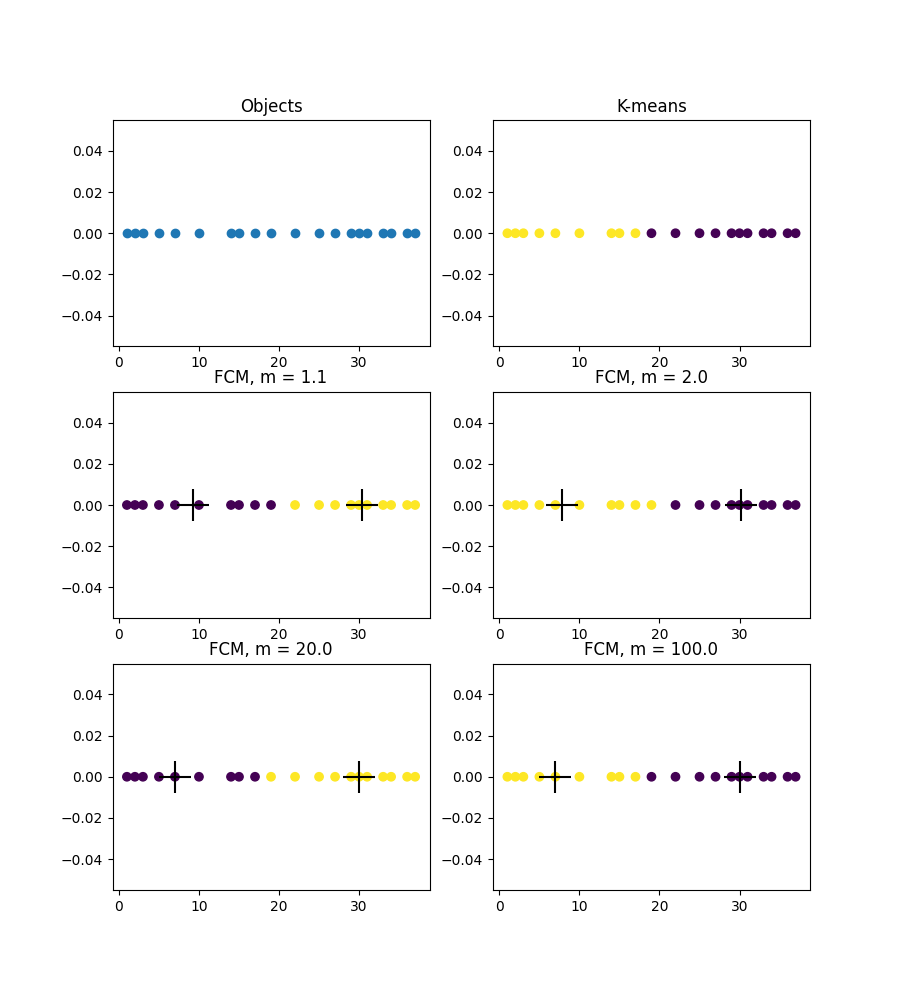
\includegraphics[width=0.8\textwidth]{fuzzy-clustering.png}
\end{figure}

Как можно заметить, расстояние между центроидами кластеров, полученных с помощью $C$-средних,
увеличивается с ростом $m$.

\subsection{Применение алгоритма}

FCM нашёл место в обработке изображений. Долгое время алгоритм $K$-средних использовался для
распознавания паттернов. Однако в связи с такими проблемами, преследующими фотосъёмку, как шум и
тени, жёсткая кластеризация не всегда способна показать удовлетворительные результаты. Для лучшего
решения подобных задач и был предложен FCM. Например, он используется при конвертации RGB в HCL.

\subsection{Задачи}

\begin{itemize}
    \item Оценить сложность алгоритма FCM.
    \item Строго показать, что $\lim\limits_{m \to 1 + 0} w_{ij} \in \{0, 1\}$.
    \item Показать, что в качестве начального приближения $w_{ij}$ нельзя брать одинаковые величины.
\end{itemize}

\subsection{Решения}

\begin{itemize}
    \item Первый шаг алгоритма занимает время $O(n)$. Далее, рассмотрим сложность каждой итерации
        цикла. Вычисление одного центроида имеет сложность $O(2n) = O(n)$. Значит, вычисление всех
        центроидов имеет сложность $O(n \cdot c)$. Расчёт одной степени принадлежности $w_{ij}$, как
        видно из формулы \eqref{fuzzy-clustering-weight}, имеет сложность $O(c)$. Тогда всех
        степеней принадлежности -- $O(n \cdot c^2)$. Вычисление целевой функции занимает время
        $O(n \cdot c)$. Таким образом, сложность одной итерации цикла составляет
        $O(n \cdot c) + O(n \cdot c^2) + O(n \cdot c) = O(n \cdot c^2)$. Поскольку условие
        $J(W, C) > \varepsilon$ эквивалентно заданию фиксированного числа итераций, то сложность
        всего цикла также составляет $O(n \cdot c^2)$. Наконец, сложность алгоритма составляет
        $O(n) + O(n \cdot c^2) = O(n \cdot c^2)$.
    \item Рассмотрим отдельное слагаемое в сумме:
        \begin{equation*}
            \lim\limits_{m \to 1 + 0} \xi^{\frac{2}{m - 1}} =
            \lim\limits_{k \to +0} \xi^{\frac{2}{k}} =
            \lim\limits_{y \to +\infty} \xi^{y}
        \end{equation*}
        Из формулы \eqref{fuzzy-clustering-weight} и определения нормы следует, что
        $\xi = \dfrac{\lVert x_i - c_j \rVert}{\lVert x_i - c_k \rVert} \geq 0$. Поэтому
        \begin{equation*}
            \lim\limits_{y \to +\infty} \xi^{y} =
            \begin{cases}
                0,\ \xi \in [0; 1) \\
                1,\ \xi = 1 \\
                +\infty,\ \xi \in (1; +\infty) \\
            \end{cases}
        \end{equation*}
        Итак, в знаменателе правой части формулы \eqref{fuzzy-clustering-weight} имеем сумму
        слагаемых, одно из которых равно 1, а из остальных каждое стремится либо к 0, либо к
        $+\infty$. Таким образом, вся сумма стремится к 1 тогда и только тогда, когда все
        слагаемые, не равные 1, стремятся к нулю, иначе -- стремится к $+\infty$. Следовательно,
        $\lim\limits_{m \to 1 + 0}w_{ij} \in \{0, 1\}$, ч.т.д.
    \item Пусть $\forall i \in \{1, \ldots, n\}, j \in \{1, \ldots, c\} \hookrightarrow w_{ij} = w$.
        Тогда, согласно формуле \eqref{fuzzy-clustering-centroid},
        \begin{equation*}
            \forall j \in \{1, \ldots, c\} \hookrightarrow c_j =
            \frac{1}{|X|}\sum\limits_{i = 1}^{|X|} x_i := z
        \end{equation*}
        Далее, по формуле \eqref{fuzzy-clustering-weight}
        \begin{equation*}
            w_{ij} = \left(\sum\limits_{k = 1}^{c} 1^{\frac{2}{m - 1}}\right)^{-1} = \frac{1}{c}
        \end{equation*}
        Итак, все $w_{ij}$ снова одинаковы, и на следующей итерации ситуация повторится, значит,
        процесс не сойдётся. Таким образом, для сходимости алгоритма необходимо выбирать различные
        начальные приближения $w_{ij}$, ч.т.д.


\section{Сети Кохонена для кластеризации}

\subsection{Задача кластеризации (обучение без учителя)}
Кластеризация — это метод обучения без учителя, при котором требуется разделить данные на группы (кластеры) на основе их сходства.  \\
\textbf{Дано:}  \\
$X_\ell = \{ x_i \}_{i=1}^{\ell}$ — обучающая выборка объектов, $x_i \in \mathbb{R}^n$ — объект с $n$ признаками.\\
$\rho^2(x, w) = || x - w ||^2$ — евклидова метрика в $\mathbb{R}^n$, которая измеряет расстояние между объектом $x$ и центром кластера $w$.\\

\textbf{Найти:} \\
Центры кластеров $w_y \in \mathbb{R}^n$, $y \in Y$ — векторные представления центров кластеров.

Правило жесткой конкуренции (WTA, Winner Takes All) говорит о том, что объект $x$ относится к тому кластеру, чьё расстояние до объекта минимально. Это правило применяется в стандартных алгоритмах кластеризации:
\[
a(x) = \arg \min_{y \in Y} \rho(x, w_y)
\]
Критерий для выбора центров кластеров — минимизация среднего внутрикластерного расстояния:
\[
Q(w; X_\ell) = \sum_{i=1}^{\ell} \rho^2(x_i, w_{a(x_i)}) \to \min_{w_y : y \in Y}
\]
Это означает, что мы стремимся минимизировать сумму квадратов расстояний от каждого объекта до ближайшего кластера.

\subsection{Сеть Кохонена (сеть с конкурентным обучением)}
Сети Кохонена относятся к нейронным сетям с конкурентным обучением. В таких сетях нейроны (кластеры) "соревнуются" за право быть ближе к объектам, и только один или несколько нейронов обновляются на каждом шаге обучения.

Структура модели — двухслойная нейронная сеть. Верхний слой — это входные данные, а нижний — это нейроны, представляющие кластеры.

\begin{figure}[h]
\centering
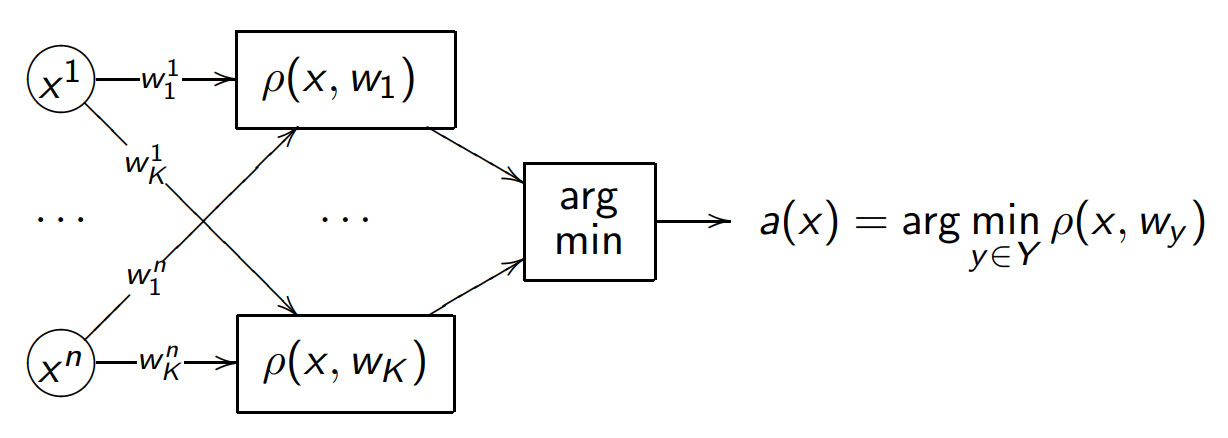
\includegraphics[width=0.7\textwidth]{scheme_kohonen.jpg}
\caption{Структура сети Кохонена}
\end{figure}

\textbf{Градиентный шаг в методе стохастического градиента (SG):}\\
Для выбранного объекта $x_i \in X_\ell$ выполняется обновление весов центра кластера $w_y$, к которому относится объект:
\[
w_y := w_y + \eta(x_i - w_y)
\]
Здесь $\eta$ — темп обучения, определяющий скорость обновления. Если объект $x_i$ относится к кластеру $y$, то центр этого кластера сдвигается в сторону объекта.

\subsection{Алгоритм обучения}
Алгоритм стохастического градиента (SG) используется для обучения сети Кохонена.\\

\textbf{Вход}: выборка $X_\ell$; темп обучения $\eta$; параметр $\lambda$.  \\
\textbf{Выход}: центры кластеров $w_y \in \mathbb{Р}^n$, $y \in Y$.

\begin{enumerate}
    \item Инициализировать центры кластеров $w_y$, $y \in Y$ случайным образом.
    \item Инициализировать оценку функционала: $Q := \sum_{i=1}^{\ell} \rho^2(x_i, w_{a(x_i)})$.
    \item Повторять:
        \begin{itemize}
            \item Выбрать объект $x_i$ из $X_\ell$ (например, случайно).
            \item Вычислить ближайший кластер: $y := \arg \min_{y \in Y} \rho(x_i, w_y)$.
            \item Градиентный шаг: $w_y := w_y + \eta(x_i - w_y)$, сдвигая центр кластера в сторону объекта.
            \item Оценить значение функционала: $Q := (1 - \lambda) Q + \lambda \rho^2(x_i, w_y)$.
        \end{itemize}
\end{enumerate}
Процесс повторяется, пока значение функционала $Q$ не стабилизируется, указывая на то, что обучение завершилось.

\subsection{Жесткая и мягкая конкуренция}
В модели с жесткой конкуренцией (WTA) только один кластер обновляется:
\[
w_y := w_y + \eta(x_i - w_y), \quad y \in Y
\]
Однако это может приводить к тому, что некоторые центры кластеров никогда не будут обновляться.

Для устранения этого недостатка используется правило мягкой конкуренции (WTM — Winner Takes Most):
\[
w_y := w_y + \eta(x_i - w_y) K(\rho(x_i, w_y)), \quad y \in Y
\]
Ядро $K(\rho)$ — неотрицательная невозрастающая функция, определяющая, насколько сильно каждый кластер обновляется в зависимости от его расстояния до объекта $x_i$. Чем дальше кластер от объекта, тем меньше его обновление.

\subsection{Задача классификации LVQ (Learning Vector Quantization)}
Learning Vector Quantization (LVQ) — это метод обучения с учителем, основанный на сетях Кохонена. Он используется для классификации, когда объекты имеют метки классов.

\textbf{Дано:}\\  
$X_\ell = \{ (x_i, y_i) \}_{i=1}^{\ell}$ — обучающая выборка, где $x_i \in \mathbb{Р}^n$ — объект, а $y_i \in Y$ — метка класса.\\
$C$ — множество кластеров, $y(c) \in Y$ — класс, к которому относится кластер $c \in C$.

\textbf{Найти:}  
Центры кластеров $w_c \in \mathbb{Р}^n$, $c \in C$ и модель классификации:
\[
a(x) = y(c(x))
\]
где $c(x)$ — ближайший кластер к объекту $x$, а $a(x)$ — предсказанный класс.

\textbf{Критерий:} \\
Задача состоит в том, чтобы минимизировать расстояния внутри кластеров для объектов одного класса и максимизировать для объектов разных классов:
\[
Q = \sum_{i=1}^{\ell} \rho^2(x_i, w_{c(x_i)}) \left( \mathbf{1}[y(c(x_i)) = y_i] - \mathbf{1}[y(c(x_i)) \neq y_i] \right) \to \min_{w_c : c \in C}
\]

\subsection{Обучаемое векторное квантование}
Метод обучаемого векторного квантования (Learning Vector Quantization, LVQ) представляет собой модель классификации, основанную на разбиении каждого класса на несколько кластеров. Это позволяет гибко описывать классы, даже если их форма сложна и не линейна. LVQ можно рассматривать как альтернативу байесовским классификаторам или методам, использующим GMM (Gaussian Mixture Model) — смесь гауссовских распределений, которые также позволяют моделировать сложные формы данных.

\begin{figure}[h]
\centering
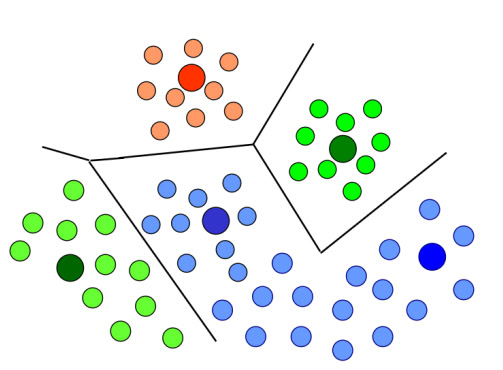
\includegraphics[width=0.7\textwidth]{clusters_kohonen.jpg}
\caption{Кластеры в сети Кохонена}
\end{figure}

\subsection{Задачи}
\subsubsection{Задача 1: Выбор метода кластеризации WTA или WTM для клиентов интернет-магазина}

\textbf{Дано:}
Рассмотрим задачу кластеризации клиентов интернет-магазина, основанную на данных о покупательском поведении. Имеются два кластера, и магазин хочет классифицировать новых клиентов, основываясь на исторических данных. Каждый клиент описывается двумя признаками: 

\begin{itemize}
    \item \textbf{Средняя сумма покупки} (в диапазоне от 100 до 500 у.е.).
    \item \textbf{Частота покупок} (в диапазоне от 1 до 20 покупок в месяц).
\end{itemize}

Цель состоит в том, чтобы выбрать метод кластеризации с использованием сетей Кохонена: \textbf{WTA (Winner-Takes-All)} или \textbf{WTM (Winner-Takes-Most)}, чтобы наилучшим образом разделить клиентов на два кластера — "активных покупателей" и "редких покупателей", исходя из вышеуказанных признаков.

Дополнительное условие: исторически известно, что у некоторых клиентов наблюдается пограничное поведение — их средняя сумма покупок нестабильна, и она может существенно колебаться, оставаясь между двумя кластерами. Частота покупок также может немного изменяться в разных месяцах.

\textbf{Данные:}
\begin{itemize}
    \item \textbf{Активные покупатели}: частота покупок — от 10 до 20, средняя сумма покупки — от 300 до 500 у.е.
    \item \textbf{Редкие покупатели}: частота покупок — от 1 до 9, средняя сумма покупки — от 100 до 300 у.е.
    \item \textbf{Пограничные клиенты}: частота покупок — от 7 до 10, средняя сумма покупки — от 250 до 350 у.е.
\end{itemize}

\textbfn{Решение:}
\textbf{Winner-Takes-All (WTA)}:
\begin{itemize}
    \item В этом методе ближайший к клиенту кластер побеждает и забирает весь вес. Это означает, что даже небольшой разброс данных не изменит решение, и каждый клиент будет жестко отнесен к тому кластеру, который находится ближе всего.
    \item \textbf{Плюсы}: Быстрое и четкое отнесение клиентов к одному кластеру. Хорошо подходит для случаев, когда данные четко разделены.
    \item \textbf{Минусы}: Не учитываются незначительные колебания данных (особенно у пограничных клиентов). Пограничные клиенты могут быть некорректно отнесены к "активным" или "редким" покупателям, что приведет к неправильной сегментации.
\end{itemize}

\textbf{Winner-Takes-Most (WTM)}:
\begin{itemize}
    \item В этом методе несколько ближайших кластеров получают долю веса в зависимости от их расстояния до клиента. Это приводит к более мягкому учету пограничных случаев.
    \item \textbf{Плюсы}: Позволяет лучше учитывать клиентов с пограничным поведением, давая возможность частичного участия в обоих кластерах. Более гибкая кластеризация, подходящая для случаев, когда данные имеют некоторое размытое распределение.
    \item \textbf{Минусы}: Может усложнить интерпретацию, так как один клиент может быть частично отнесен сразу к нескольким кластерам.
\end{itemize}

\textbf{Оценка данных}: 
Клиенты, которые четко относятся к одной из двух категорий (активные или редкие покупатели), имеют устойчивые значения признаков, что позволяет эффективно использовать метод WTA. 

\textbf{Проблема возникает с пограничными клиентами}, чьи значения частоты покупок и средней суммы находятся между кластерами. В случае использования WTA такие клиенты могут быть жестко отнесены к одному кластеру, даже если их поведение не является достаточно устойчивым для точного отнесения к активным или редким покупателям. Это может исказить результаты сегментации.

\textbf{Заключение:}
В данной задаче \textbf{WTM (Winner-Takes-Most)} является более предпочтительным методом, так как он позволяет учесть пограничное поведение клиентов и сгладить влияние неустойчивых данных. В случае применения WTA, пограничные клиенты будут жестко отнесены к одному кластеру, что приведет к снижению точности кластеризации. Таким образом, метод WTM будет лучшим выбором, поскольку он дает возможность учитывать неопределенность и вариативность данных клиентов.

\subsubsection{Задача 2: Выбор метода кластеризации для различных задач}

\textbf{Дано:}
Перед вами стоит задача выбора метода кластеризации для разделения данных на несколько групп. Рассмотрены следующие методы кластеризации:
\begin{itemize}
    \item \textbf{Нейронная сеть Кохонена}.
    \item \textbf{K-средних (K-means)}.
    \item \textbf{Иерархическая кластеризация (Hierarchical Clustering)}.
\end{itemize}

Для каждого метода необходимо привести его плюсы и минусы, а также обосновать, в каких случаях каждый из методов будет предпочтителен.

\subsubsection{Решение:}

\textbf{1. Нейронная сеть Кохонена}:
\begin{itemize}
    \item \textbf{Плюсы:}
    \begin{itemize}
        \item \textbf{Сокращение размерности:} сеть Кохонена автоматически проецирует многомерные данные на двумерную решетку, что позволяет визуализировать высокоразмерные данные. Это особенно полезно для анализа сложных данных.
        \item \textbf{Нелинейное разделение:} сеть Кохонена может кластеризовать данные, которые не разделяются линейно, что делает его более гибким для задач с неявными границами между кластерами.
        \item \textbf{Интерпретируемость:} сеть Кохонена создает топологическую карту, где схожие объекты оказываются близко друг к другу, что позволяет увидеть, какие данные похожи и как распределены кластеры.
        \item \textbf{Мягкая конкуренция:} Сети Кохонена поддерживают мягкую конкуренцию между нейронами, что позволяет учитывать схожесть объектов в соседних кластерах.
    \end{itemize}
    \item \textbf{Минусы:}
    \begin{itemize}
        \item \textbf{Трудоемкость настройки:} Требует тщательной настройки параметров, таких как размеры решетки и скорость обучения.
        \item \textbf{Чувствительность к выбору начальных весов:} Результаты могут зависеть от начальной инициализации, что иногда приводит к неоптимальным решениям.
        \item \textbf{Трудности с выбором числа кластеров:} Метод не предоставляет четкого способа выбора количества кластеров.
    \end{itemize}
\end{itemize}

\textbf{2. Метод K-средних (K-means)}:
\begin{itemize}
    \item \textbf{Плюсы:}
    \begin{itemize}
        \item \textbf{Простота и быстрота:} K-means прост в реализации и эффективен при больших объемах данных.
        \item \textbf{Легкость интерпретации:} Метод делит данные на четкие кластеры, что упрощает анализ и интерпретацию результатов.
        \item \textbf{Хорошо работает с линейно разделимыми данными:} K-means подходит для данных, где кластеры можно разделить прямыми границами.
    \end{itemize}
    \item \textbf{Минусы:}
    \begin{itemize}
        \item \textbf{Чувствительность к форме кластеров:} Метод плохо работает с данными, где кластеры имеют сложную форму или сильно перекрываются.
        \item \textbf{Чувствительность к выбросам:} Выбросы могут сильно повлиять на центроиды кластеров.
        \item \textbf{Необходимость выбора числа кластеров:} Требуется заранее задавать количество кластеров, что не всегда очевидно.
    \end{itemize}
\end{itemize}

\textbf{3. Иерархическая кластеризация (Hierarchical Clustering)}:
\begin{itemize}
    \item \textbf{Плюсы:}
    \begin{itemize}
        \item \textbf{Гибкость в выборе числа кластеров:} Иерархическая кластеризация позволяет на любом этапе "отрезать" дерево и выбрать нужное количество кластеров.
        \item \textbf{Не требует заранее определенного числа кластеров:} Этот метод не требует от пользователя указания числа кластеров заранее.
        \item \textbf{Дает информацию о структуре данных:} Результаты представлены в виде дендрограммы, что позволяет увидеть иерархию кластеров и их отношения.
    \end{itemize}
    \item \textbf{Минусы:}
    \begin{itemize}
        \item \textbf{Высокая вычислительная сложность:} Алгоритм может быть неэффективен для очень больших наборов данных.
        \item \textbf{Чувствительность к шуму:} Иерархические методы могут быть чувствительны к выбросам и шуму в данных.
        \item \textbf{Сложность в интерпретации:} Дендрограмма может быть трудной для интерпретации, особенно если структура данных сложная.
    \end{itemize}
\end{itemize}

\subsubsection{Задача 3: Сравнение архитектур для кластеризации}

\textbf{Дано:}

Представьте, что вам нужно применить два различных подхода для кластеризации данных: один с использованием сети Кохонена, а другой с использованием автокодировщика (autoencoder). Оба подхода решают задачу кластеризации на данных о изображениях. Задание состоит в том, чтобы указать основные архитектурные отличия между сетью Кохонена и автокодировщиком, которые могут повлиять на результаты кластеризации, и объяснить, как эти различия влияют на процесс обучения и кластеризацию.

\textbf{Решение:}

\textbf{1. Сеть Кохонена:}

\begin{itemize}
    \item \textbf{Архитектура:} Это тип нейронной сети, состоящий из одномерной или двумерной решетки нейронов, каждый из которых имеет веса, соответствующие входным данным. На вход сети подаются данные, и нейрон, чьи веса наиболее похожи на входной вектор, становится «победителем» (наиболее конкурентоспособным). Нейроны, расположенные рядом с победителем, также обновляют свои веса, что стимулирует близкие кластеры.
    \item \textbf{Обучение:} Используется метод обучения без учителя, с конкуренцией между нейронами (жесткая конкуренция). Кластеры формируются на основе минимизации расстояния между нейронами и входными векторами.
    \item \textbf{Отличие:} Основной особенностью сети Кохонена является принцип конкуренции, где нейроны обучаются на основе «победителя», и близкие нейроны обновляют свои веса. Это позволяет сетке создавать топологически осмысленные кластеры.
\end{itemize}

\textbf{2. Автокодировщик (autoencoder):}

\begin{itemize}
    \item \textbf{Архитектура:} Автокодировщик состоит из двух частей: энкодера и декодера. Энкодер принимает входные данные и сжимает их в более низкоразмерное пространство (латентное пространство), а декодер восстанавливает данные обратно в исходное пространство. Автокодировщики могут быть обучены с использованием метода обратного распространения ошибки для минимизации разницы между входом и восстановленным выходом.
    \item \textbf{Обучение:} Автокодировщик использует метод обучения с учителем (по сути, обучается на восстановление данных), что отличается от обучения без учителя в сети Кохонена. Он минимизирует ошибку восстановления, а не конкуренцию между нейронами.
    \item \textbf{Отличие:} Главным отличием является наличие явной цели для восстановления входных данных через латентное пространство. Это приводит к тому, что автокодировщик учит сеть выделять наиболее значимые признаки для восстановления данных, что влияет на кластеризацию.
\end{itemize}

\section*{Трансдуктивный метод опорных векторов TSVM}

\subsection{Общее описание метода}

Трансдуктивный метод опорных векторов (TSVM) является частью методов обучения с учителем, которые применяются к задачам, где часть данных размечена, а часть — нет. В отличие от классического метода опорных векторов (SVM), который использует только размеченные данные, TSVM может эффективно работать как с размеченными, так и с неразмеченными данными.

Пусть у нас есть данные:
\[
    X_k = \{x_1, x_2, \dots, x_k\} \quad \text{— размеченные данные},
\]
\[
    y_k = \{y_1, y_2, \dots, y_k\} \quad \text{— метки для размеченных данных},
\]
\[
    U = \{x_{k+1}, x_{k+2}, \dots, x_\ell\} \quad \text{— неразмеченные данные}.
\]

Цель метода — найти классификатор \( a(x, w) \), который минимизирует общую ошибку на размеченных данных, а также штрафует классификатор за неопределенность на неразмеченных данных.

Определение классификатора:
\[
    a(x, w) = \text{sign}(\langle w, x \rangle - w_0).
\]

Функционал потерь для TSVM включает обе ошибки:
\[
    \sum_{i=1}^{k} L(a(x_i, \textcolor{red}{w}), y_i) + \lambda \sum_{i=k+1}^{\ell} L_U(a(x_i, \textcolor{red}{w})) \to \min_\textcolor{red}{w},
\]
где:\\
 \( L(a(x_i, \textcolor{red}{w}), y_i) \) — функция потерь для размеченных данных,\\
 \( L_U(a(x_i, \textcolor{red}{w})) \) — штрафная функция для неразмеченных данных,\\
 \( \lambda \) — параметр, регулирующий важность штрафа за неопределенность.\\

Суть в том, чтобы параметризовать $\textcolor{red}{w}$ в двух критериях. 
\subsection{Идея для штрафа из классификатора SVM}
    Пусть у нас есть линейный классификатор на два класса \( Y = \{-1, 1\} \):
    \[
        a(x) = \text{sign} \left( \langle w, x \rangle - w_0 \right), \quad w, x \in \mathbb{R}^n
    \]
    
    \textbf{Напоминание: Отступ (margin) объекта \( x_i \)} — это мера того, насколько правильно классифицирован объект, с учетом расстояния до разделяющей гиперплоскости. Для объекта \( x_i \) с меткой \( y_i \) отступ определяется как:
    \[
        M_i(w, w_0) = \left( \langle w, x_i \rangle - w_0 \right) y_i.
    \]
    Если отступ положителен и больше 1, объект классифицирован правильно и лежит за пределами разделяющей полосы, что свидетельствует о хорошей уверенности в классификации. Если отступ меньше 1, объект либо лежит внутри разделяющей полосы, либо ошибочно классифицирован.

    \textbf{Задача обучения} весов \( w, w_0 \) нашего классификатора на размеченной выборке ставится следующим образом:
    \[
        Q(w, w_0) = \sum_{i=1}^{k} \left( 1 - M_i(w, w_0) \right)_+ + \frac{1}{2C} \|w\|^2 \to \min_{w, w_0}.
    \]
    где функция потерь \( L(M) = (1 - M)_+ \) штрафует за объекты, которые оказываются слишком близко к разделяющей гиперплоскости или ошибочно классифицированы (т.е. \( M_i < 1 \)).

    \vspace{1em}
    \textbf{Идея для метода TSVM}

    Таким образом получаем идею, реализованную в методе трансдуктивной SVM (TSVM), где используется штраф для объектов, которые неразмечены. В TSVM требуется учесть неопределенные данные, вводя штраф за попадание объекта внутрь разделяющей полосы, что настраивается параметром \( \gamma \). Для этого используется модифицированная функция штрафа для неразмеченных данных:
    \[
        L_U(M) = \left( 1 - |M| \right)_+,
    \]
    где \( M \) — это отступ объекта. Такой штраф вводится для того, чтобы минимизировать неопределенность классификации и корректно учитывать информацию о неразмеченных данных в процессе обучения модели.
    
    \begin{figure}[ht]
    \centering
    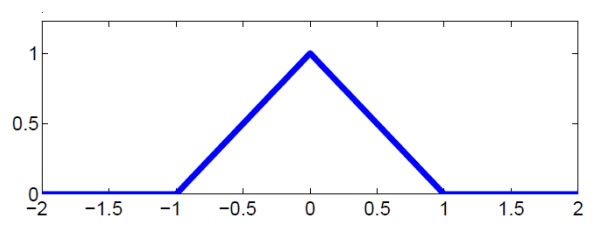
\includegraphics[width=0.5\textwidth]{MLbook/chapters/clustering/png/TSVMLoss.jpg}
    \caption{Вид функции штрафа для неразмеченных данных.}
    \end{figure}

\begin{figure}[ht]
    \centering
    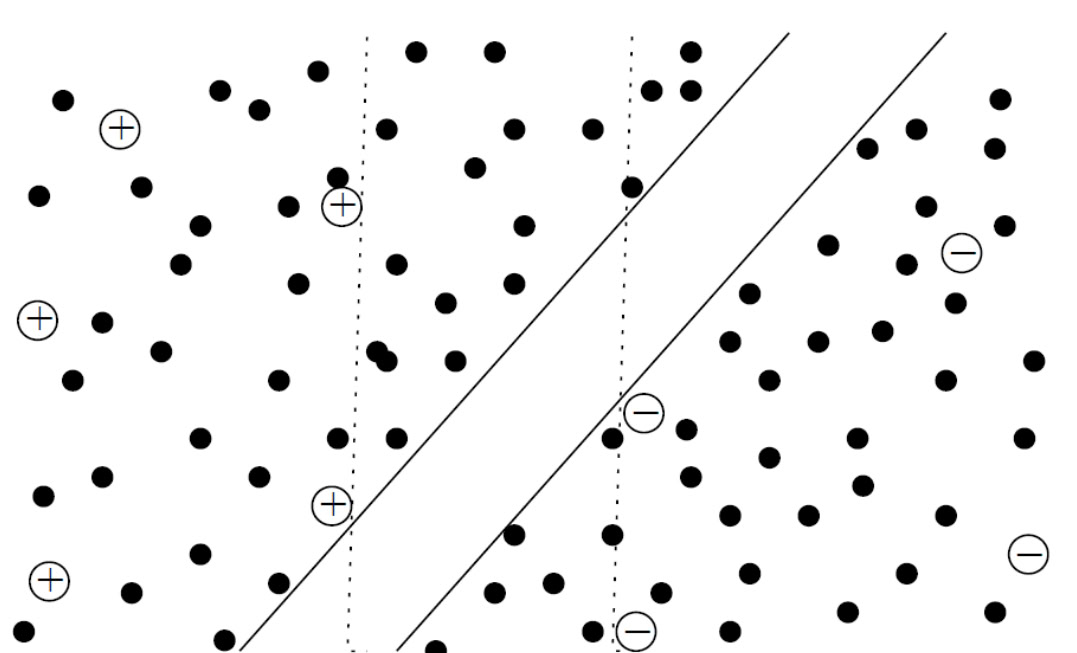
\includegraphics[width=0.5\textwidth]{MLbook/chapters/clustering/png/ClassifierData.jpg}
    \caption{Пример распределения точек около границы.}
\end{figure}

\subsection{Математическое описание трансдуктивной задачи}
С математической точки зрения новая трансдуктивная задача описывается следующим образом:

\begin{equation}
    Q(w, w_0) = \sum_{i=1}^{k} \left( 1 - \textcolor{red}{M_i(w, w_0)} \right)_+ + \frac{1}{2C} \|w\|^2 + \gamma \sum_{i=k+1}^{\ell} \left( 1 - |\textcolor{red}{M_i(w, w_0)}| \right)_+ \to \min_{\textcolor{red}{w, w_0}}.
\end{equation}

Данный подход позволяет учитывать как известные, так и неизвестные (неразмеченные) данные для более точного обучения модели.

\textbf{Основные преимущества и недостатки TSVM}:
\begin{itemize} 
    \item \textbf{Преимущества:} 
    \begin{itemize} 
        \item Как и в обычном SVM, можно использовать ядра для работы с нелинейными задачами. 
        \item Имеются эффективные реализации, которые позволяют работать с большими объемами данных. 
    \end{itemize}
        
    \item \textbf{Недостатки:}
    \begin{itemize}
        \item Задача оптимизации TSVM не является выпуклой, что делает методы оптимизации более сложными.
        \item Решение может быть неустойчивым, если нет области разреженности в данных.
        \item Требуется настройка двух параметров: \( C \) и \( \gamma \).
    \end{itemize}

    \item \textbf{Применение:} 
    TSVM используется в задачах, где важно учитывать как размеченные, так и неразмеченные данные для повышения точности классификации. Это делает метод особенно полезным для работы с большими объемами неразмеченных данных, которые часто встречаются в реальных приложениях.
\end{itemize}

\subsection{Задачи}
\subsubsection*{Задача 1}
\textbf{Условие:} Покажите на примере двух точек $(1/3, 1/3)$ и $(-2, -2)$ и линейного классификатора  с $w_0 = 0, w_1 = 1, w_2 = 1$ как именно считается модифицированная функция штрафа $L_U(M)$. \\
\textbf{Решение:}
Классифицирующей поверхностью в нашем случае является прямая $y = -x$ с соответствующей полосой, поэтому можем взять точки $(1/3, 1/3)$ и $(-2, -2)$ для того, чтобы продемонстрировать требуемое. Для них соответственно получаем:
\[
    L_1 = (1 - |(1/3*1 + 1/3*1 + 0)|)_+ = 1/3
\]

\[
    L_2 = (1 - |((-2)*1 + (-2)*1 + 0)|)_+ = 0
\]
\[
    L_{all} = 1/3 + 0 = 1/3
\]
Мы умножаем M на 1 вне зависимости от знака класса, т.к. в формуле стоит модуль, это опустили.
\subsubsection*{Задача 2}
\textbf{Условие:}
В рамках предыдущей задачи покажите, что для классификатора с теми же $w_1, w_2$, но $w_0 = -1$ получившийся штраф будет меньше. Соответствует ли это лучшей разделимости точек? Продемонстрируйте картинки с пояснениями.\\
\textbf{Решение:}
Аналогично будем иметь:
\[  
    L_1 = (1 - |(1/3*1 + 1/3*1 + 1)|)_+ = 0
\]

\[
    L_2 = (1 - |((-2)*1 + (-2)*1 + 1)|)_+ = 0
\]

\[
    L_{all} = 0 + 0 = 0
\]
Таким образом штраф уменьшился, и как видно из картинок, точки стали распределены вне линии разделения:
\begin{figure}[ht]
    \centering
    \begin{minipage}{0.45\textwidth}
        \centering
        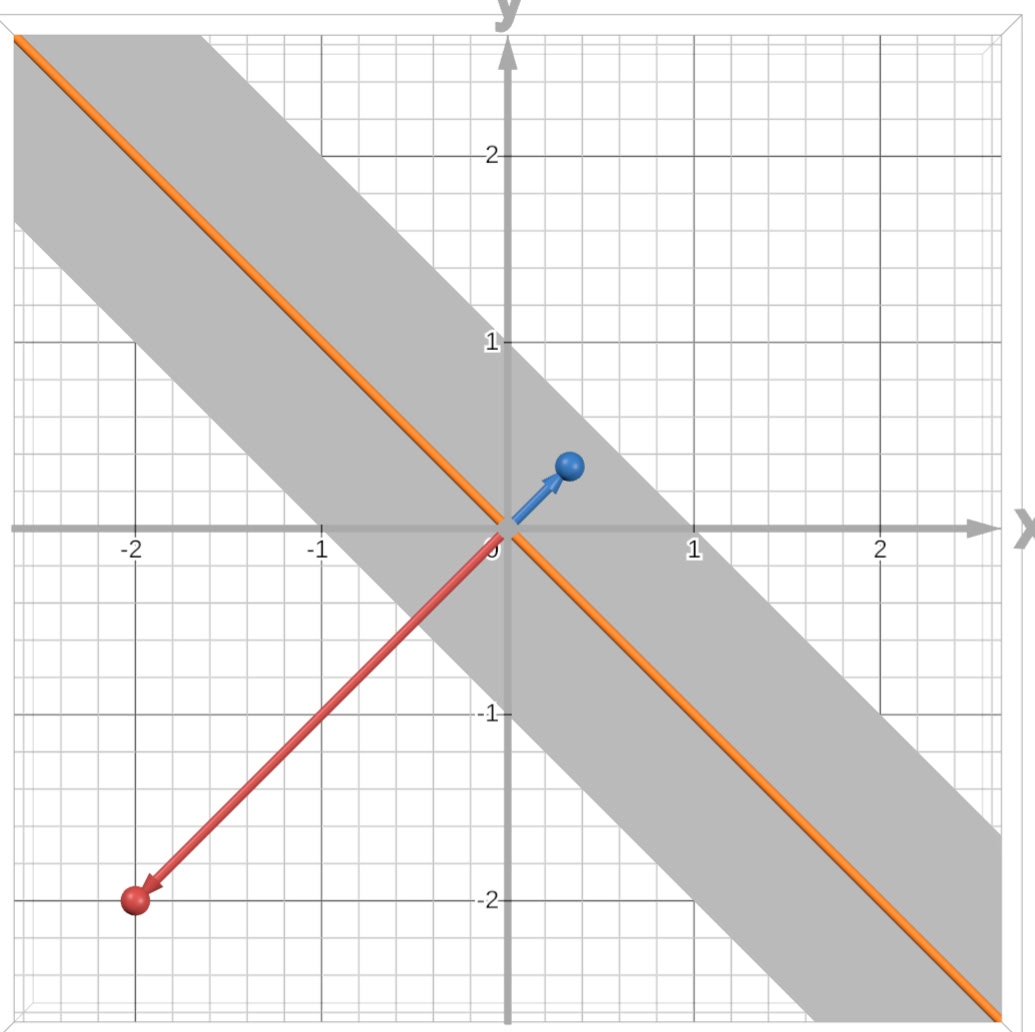
\includegraphics[width=0.9\textwidth]{MLbook/chapters/clustering/png/TSVM_3task1.jpg}
        \caption{$w_0 = 0$}
    \end{minipage}
    \hfill
    \begin{minipage}{0.45\textwidth}
        \centering
        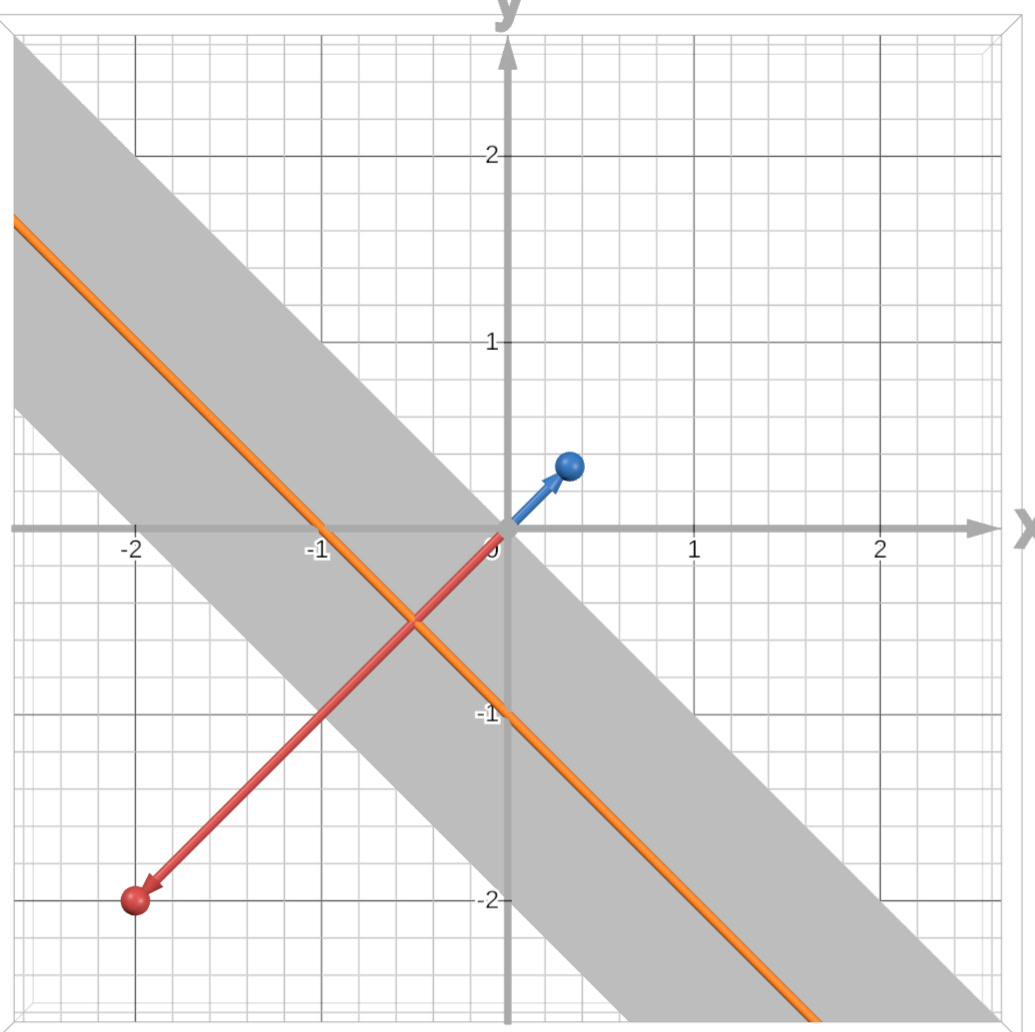
\includegraphics[width=0.9\textwidth]{MLbook/chapters/clustering/png/TSVM_3task2.jpg}
        \caption{$w_0 = -1$}
    \end{minipage}
\end{figure}

\subsubsection*{Задача 3}
\textbf{Условие:}
Можно ли использовать метод TSVM для постепенного самообучения, размечая данные по мере их поступления? Какие преимущества и недостатки могут быть у такого подхода?\\
\textbf{Решение:}\\
\textbf{Преимущества:}
\begin{itemize}
    \item \textbf{Эффективное использование неразмеченных данных:} Постепенное добавление размеченных данных на основе текущих предсказаний TSVM позволяет улучшить модель по мере поступления новых данных. Это может быть полезно, если размечать данные вручную дорого или занимает много времени.
    \item \textbf{Гибкость в обучении:} Метод TSVM может адаптироваться к новым данным и улучшать границу классификации, не требуя полного перерасчета модели с нуля каждый раз. Это особенно полезно в задачах, где данные поступают по мере времени (например, в потоках информации).
    \item \textbf{Обучение на малых объемах данных:} TSVM позволяет начать с небольшого набора размеченных данных и постепенно расширять его, используя информацию о неразмеченных примерах. Это важно, когда размеченные данные труднодоступны или ограничены.
\end{itemize}\\
\textbf{Недостатки:}
\begin{itemize}
    \item \textbf{Риски неправильной разметки:} Одной из проблем такого подхода является риск неверной или неточной разметки данных в процессе самообучения. Если начальная модель не обладает высокой точностью, ошибки в разметке могут привести к накоплению ошибок в дальнейшем обучении.
    \item \textbf{Проблемы с неопределенностью:} Неопределенные данные (примеры, которые находятся близко к границе принятия решения) могут быть ошибочно размечены. TSVM решает эту проблему через регуляризацию, но все же может столкнуться с трудностями при обработке сложных случаев, когда граница классификации неясна.
    \item \textbf{Зависимость от начальных данных:} Результат обучения сильно зависит от начального набора размеченных данных. Если эти данные не являются репрезентативными, то модель может в дальнейшем плохо обрабатывать новые примеры.
\end{itemize}
